\chapter{Integral de Lebesgue}
Una vez definida la medida en $\mathbb{R}^n$, tenemos todos los ingredientes necesarios para desarrollar una teoría de la integrabilidad sólida. Durante este capítulo se va a desarrollar la Integral de Lebesgue, relacionar dicha integral con la integral de Riemann y estudiar las propiedades de las que goza dicho objeto matemático.

\section{Definición de Integral}
La definición de la integral de Lebesgue posibilita extender la Integral de Riemann y establecer un cimiento sólido para todas aquellas áreas matemáticas que se nutren de la integración y que poseen situaciones peculiares que hacen las integrales de Riemann inservibles.

\begin{obs}
Recordemos que llamamos función simple a una función con la estructura:
$$\varphi = \sum_{k=1}^{m} \alpha_k \chi_{E_k}$$
Dicha función cumple que:
\begin{itemize}
    \item Es una función medible.
    \item Solo toma un número finito de valores.
    \item Cualquier función $\varphi$ que sea medible y solo tome un número finito de valores $(\beta_1, \ldots, \beta_r)$ es una función simple, puesto que podemos expresar dicha función como:
\begin{align*}
E_j = \varphi^{-1}\left(\{\beta_j\}\right) \text{, medible} & & \varphi = \sum_{k=1}^{r} \beta_j \chi_{E_j} \Rightarrow \varphi \text{ es simple.}
\end{align*}
\end{itemize}
\end{obs}

\begin{defi}[Integral]
Sea $\varphi$ función simple no negativa:
$$\varphi = \sum_{k=1}^{m} \alpha_k \cdot \chi_{E_k} \mbox{ donde } \left(\alpha_k > 0\right)$$
Definimos la \textbf{integral} de dicha función como:
$$I\left(\varphi\right) = \sum_{k=1}^{m} \alpha_k \mu\left(E_k\right)$$
\end{defi}

\begin{obs}
Como la medida de dichos conjuntos puede ser infinito y los valores $\alpha_k = 0$, es necesario que definamos $0 \cdot \left(+ \infty\right) = 0$ para poder dar una definición consistente de $I\left(\varphi\right) \in \left[0, +\infty\right]$.
\end{obs}


\begin{prop}
Sea $\varphi$ función simple, es posible escribir dicha función de distintas formas:
$$\varphi = \sum_{i=1}^{m} \alpha_i \chi_{E_i} = \sum_{i=1}^{p} \beta_i \chi_{D_i}$$
entonces la integral coincide para cualquiera que sea la forma escogida:
$$I(\varphi) = \sum_{i=1}^{m} \alpha_i \mu\left(E_i\right) = \sum_{i=1}^{p} \beta_i \mu\left(D_i\right)$$
luego la integral tiene una definición consistente.
\end{prop}
\begin{demo}
La demostración se deja como ejercicio de las hojas, se trata de utilizar que entre dos cualesquiera puedo pasar por la forma canónica y esta integral es la de la definición.
\end{demo}

\begin{prop}
\begin{enumerate}
    \item Sea $c > 0$ y $\varphi$ simple no negativa, entonces $I\left(c\cdot \varphi\right) = c\cdot I\left(\varphi\right)$.
    \item Sean $\varphi, \psi$ simples no negativas, entonces $I\left(\varphi + \psi\right) = I\left(\varphi\right) + I\left(\psi\right)$
    \item Si $\varphi \le \psi$ c.t.p, entonces $I\left(\varphi\right) \le I\left(\psi\right)$
    \item Si $\varphi = \psi$ c.t.p, entonces $I\left(\varphi\right) = I\left(\psi\right)$
\end{enumerate}
\end{prop}
\begin{obs}
Los conjuntos no tienen porque ser intervalos, si fuese este el caso sería, en el fondo, integrabilidad Riemann.
\end{obs}

\begin{prop}
Si $\varphi$ es una función simple no negativa y $A_1 \cap A_2 = \emptyset$:
\[
I \left( \varphi \left( x \right) \right) = I \left( \varphi \left( x \right) \cdot A_1 \right) + I \left( \varphi \left( x \right) \cdot A_2 \right)
\]
\end{prop}

\begin{defi}[Integral de Lebesgue]
Sea $f: \mathbb{R}^n \rightarrow \left[0, +\infty\right]$ una función medible, definimos la \textbf{integral de Lebesgue de $f$} de la siguiente\footnote{La definición no cambia si las funciones $\varphi \leq f$ en c.t.p.} forma:
$$\int_{\mathbb{R}^n}f \ d\mu = \sup_{\varphi \leq f} I\left(\varphi\right) \in \left[0, +\infty\right]$$
Donde las funciones $\varphi$ son simples no negativas.
\end{defi}

\begin{prop}
Sea $\varphi$ simple no negativa, la integral de Lebesgue coincide con la integral definida para este tipo de funciones:
$$\int_{\mathbb{R}^n}\varphi \ d \mu = I\left(\varphi\right)$$
\end{prop}
\begin{demo}
En primer lugar, la primera desigualdad la tenemos por ser el supremo de las Integrales de las funciones simples menores o iguales que $\varphi$, es decir:
$$\varphi \le \varphi \Rightarrow I\left(\varphi\right) \leq \sup_{\psi \leq \varphi} I(\psi) = \int_{\mathbb{R}^n} \varphi \ d \mu $$
Si $\int_{\mathbb{R}^n} \varphi \ d \mu = +\infty$, entonces tenemos que:
$$\forall M > 0,\ \exists \psi \le \varphi: I\left(\psi\right) \ge M \Rightarrow M \le I\left(\psi\right) \le I\left(\varphi\right) \Rightarrow \forall M > 0: I\left(\varphi\right) \ge M \Rightarrow I\left(\varphi\right) = +\infty$$
Si $\int_{\mathbb{R}^m}\varphi \ d \mu < +\infty$, entonces tenemos que:
$$\forall \varepsilon > 0,\ \exists \psi \le \varphi: I\left(\psi\right) \ge \int_{\mathbb{R}^n}\varphi \ d \mu - \varepsilon \Rightarrow I\left(\varphi\right) \ge I(\psi) \geq  \int_{\mathbb{R}^n}\varphi \ d \mu - \varepsilon \Rightarrow I\left(\varphi\right) \ge \int_{\mathbb{R}^n}\varphi \ d \mu$$
\end{demo}

\begin{prop}
Sean $f, g: \mathbb{R}^n \rightarrow \left[0, +\infty\right]$ dos funciones medibles tal que $f \le g$ c.t.p., entonces:
$$\int_{\mathbb{R}^n}f \ d \mu \le \int_{\mathbb{R}^n}g \ d \mu.$$
\end{prop}
\begin{demo}
Se deja como ejercicio.
\end{demo}

\begin{coro}
Sean $f, g: \mathbb{R}^n \rightarrow \left[0, +\infty\right]$ dos funciones medibles tal que $f = g$ c.t.p., entonces:
$$\int_{\mathbb{R}^n}f \ d \mu = \int_{\mathbb{R}^n} g \ d \mu$$
\end{coro}

\begin{defi}[Integral en un conjunto]
Sea $A \subset \mathbb{R}^n$ un conjunto medible y $f: A \rightarrow \left[0, +\infty\right]$ una función medible, entonces definimos \textbf{la integral de $f$ sobre $A$} como:
$$\int_A f \ d \mu = \int_{\mathbb{R}^n}f \cdot \chi_{A} \ d \mu$$
\end{defi}

\begin{obs}
En general se trabajará con funciones no infinitas para evitar que la integral sea infinita trivialmente.
\end{obs}

\begin{prop}
Si $f:\mathbb{R}^n\rightarrow \mathbb{R}$ es una función medible, entonces el conjunto $\{(x, f(x))\}$ que definimos como la gráfica $f$ tiene medida $0$.
\end{prop}

\begin{lema}
Sea $\varphi$ función simple no negativa y $\{A_k\}_{k=1}^{\infty}\uparrow A$ suc. creciente $\left(A_k \subset A_{k+1} : \bigcup_{k \in \mathbb{N}} A_k = A\right)$ de conjuntos medibles convergentes a $A$, entonces:
$$\int_A \varphi \ d \mu = \lim_{k\rightarrow\infty} \int_{A_k} \varphi \ d \mu.$$
\end{lema}
\begin{demo}
Tenemos que $\varphi = \sum_{j=1}^{m} \alpha_j \cdot \chi_{E_j}$, entonces:
$$\lim_{k\rightarrow\infty} \int_{A_k} \varphi \ d \mu = \lim_{k\rightarrow\infty} \int_{\mathbb{R}^n}\varphi \cdot \chi_{A_k} \ d \mu =$$
$$= \lim_{k\rightarrow\infty} \int_{\mathbb{R}^n} \left(\sum_{j=1}^{m} \alpha_j \cdot \chi_{E_j}\cdot \chi_{A_k}\right) \ d \mu= \lim_{k\rightarrow\infty} \int_{\mathbb{R}^n} \left(\sum_{j=1}^{m} \alpha_j \cdot \chi_{E_j \cap A_k}\right) d \mu = $$
$$= \lim_{k\rightarrow\infty} \sum_{j=1}^{m} \left( \alpha_j \int_{\mathbb{R}^n} \chi_{E_j \cap A_k} d \mu \right) = \lim_{k\rightarrow\infty} \sum_{j=1}^{m} \alpha_j \cdot \mu\left(E_j \cap A_k\right) = \sum_{j=1}^{m} \alpha_j \cdot \lim_{k\rightarrow\infty} \mu\left(E_j \cap A_k\right) = $$
$$= \sum_{j=1}^{m} \alpha_j \cdot \mu\left(E_j \cap A\right) = \sum_{j=1}^{m} \left(\alpha_j \int_{\mathbb{R}^n} \chi_{E_j \cap A} \ d \mu\right) = \int_{\mathbb{R}^n}\sum_{j=1}^{m} \alpha_j \chi_{E_j} \chi_{A} \ d \mu= \int_{\mathbb{R}^n} \varphi \cdot \chi_A \ d \mu = \int_A \varphi \ d \mu$$
\end{demo}

\subsection{Propiedades de la integral}
Vamos a demostrar las operaciones y propiedades analíticas que tiene esta nueva definición de integral que se ha dado.

\begin{theo}[Convergencia Monótona]
Supongamos una sucesión creciente de funciones $\{f_k\}_{k=1}^\infty \uparrow f$ convergente\footnote{Esto quiere decir que $f_k \leq f_{k+1}$ y $\lim_{k\rightarrow\infty} f_k(x) = f(x)$ de forma puntual} a $f$ donde cada función $f_k: \mathbb{R}^n \rightarrow \left[0, +\infty\right]$ es medible, entonces:
$$\int_{\mathbb{R}^n}f \ d \mu = \lim_{k\rightarrow\infty} \int_{\mathbb{R}^n} f_k \ d \mu$$
El teorema también es válido si la convergencia es en c.t.p.
\end{theo}
\begin{demo}
Por la monotonía de la sucesión, tenemos que:
$$\forall k \in \mathbb{N}: f_k \le f \Rightarrow \int_{\mathbb{R}^n} f_k \ d \mu \le \int_{\mathbb{R}^n} f \ d \mu$$
Por tanto, tenemos asegurada la convergencia de la sucesión de integrales por ser acotada superiormente y creciente:
$$\left\lbrace \int_{\mathbb{R}^n} f_k \ d \mu \right\rbrace_{k=1}^{\infty}\uparrow \ \wedge \ \exists \lim_{k\rightarrow\infty} \int_{\mathbb{R}^n} f_k \ d \mu \le \int_{\mathbb{R}^n}f \ d \mu$$

Fijamos $\varphi \le f$ simple no negativa y un $c < 1$. De este modo, definimos la siguiente sucesión de conjuntos:
$$A_k = \{x \in \mathbb{R}^n: c\cdot \varphi\left(x\right) \leq f_k\left(x\right)\}$$
Dicho conjunto es medible para cada k por ser el conjunto de puntos donde una función vale más que 0.

Por ser creciente la sucesión de funciones, es decir, $f_k \le f_{k+1}$, entonces tenemos que:
$$A_k \subset A_{k+1} \Rightarrow \{A_k\}_{k=1}^{\infty} \uparrow \mathbb{R}^n \mbox{ ya que }\bigcup_{n\in \mathbb{N}}A_k = \mathbb{R}^n$$

Si $f(x) = \infty$, entonces tenemos que:
$$\lim_k f_k \left(x\right) = +\infty \Rightarrow c\cdot \varphi\left(x\right) \in \mathbb{R},\ \exists k \in \mathbb{N} : c\cdot \varphi\left(x\right) < f_k\left(x\right) \Rightarrow x \in A_k$$
Por otro lado, si tenemos que $0 < f\left(x\right) < \infty $, entonces:
$$\varphi\left(x\right) \le f\left(x\right) \Rightarrow c\cdot \varphi\left(x\right) < f\left(x\right) \Rightarrow \lim_{k\rightarrow\infty} f_k\left(x\right) = f\left(x\right) \Rightarrow \exists k \in \mathbb{N} : c\cdot \varphi\left(x\right) < f_k\left(x\right)\Rightarrow x\in A_k$$

Por tanto, por el lema anterior, al tener la sucesión creciente de los $A_k$, tenemos que:
$$c \cdot \int_{\mathbb{R}^n}\varphi \ d \mu = c\cdot \int_{\mathbb{R}^n \setminus \{x : f\left(x\right) = 0\}}\varphi \ d \mu = \int_{\mathbb{R}^n \setminus \{x : f\left(x\right) = 0\}} c  \cdot \varphi \ d \mu = $$
$$=\lim_{k\rightarrow\infty} \int_{A_k} c \cdot \varphi \ d \mu \le \lim_{k\rightarrow\infty} \int_{A_k} f_k \ d \mu \le \lim_{k\rightarrow\infty} \int_{\mathbb{R}^n} f_k \ d \mu$$
De este modo, como el $c$ es arbitrario, si se hace tender a $1$, tenemos que:
$$\int_{\mathbb{R}^n} \varphi \ d \mu \le \lim_{k\rightarrow\infty} \int_{\mathbb{R}^n} f_k \ d \mu \stackrel{\forall \varphi}{\Rightarrow} \int_{\mathbb{R}^n}f \ d \mu = \sup_{\varphi \le f} \int_{\mathbb{R}^n}\varphi \ d \mu \le \lim_{k\rightarrow\infty} \int_{\mathbb{R}^n}f_k \ d \mu$$
Y ya tendríamos demostradas las dos desigualdades.
\end{demo}

\begin{obs}
Este resultado sigue siendo cierto si se toman las hipótesis solo en c.t.p. Si ocurriese que $f_k \leq f$ no se cumpliera en un conjunto de medida nula, tomamos $f'_k$ que vale $f_k$ en todos los puntos donde se cumple y 0 en los que no. Como, por definición, $f_k = f'_k$ en c.t.p. la integral es la misma y la demostración no se ve alterada.
\end{obs}

\begin{theo}
Sea $f: \left[a, b\right] \rightarrow \mathbb{R}^+$ una función acotada e integrable Rienmann, entonces $f$ es integrable Lebesgue y verifica:
$$\int_{\left[a, b\right]}f \ d \mu = \int_a^b f\left(x\right)\ dx$$
\end{theo}
\begin{demo}
Por ser acotada, $\exists M > 0: f \le M\chi_{\left[a, b\right]}$, lo que implica que $\int f \ d \mu \leq \int M \cdot \chi_{[a,b]}$, es decir, que es integrable Lebesgue.

Además, por ser integrable Riemann, tenemos que:
$$\int_a^b f\left(x\right)dx = \sup_{P \in \wp} L\left(f, P\right) \Rightarrow \exists \{P_k\}_{k=1}^{\infty} : P_k \leq P_{k+1} : \int_a^b f\left(x\right) \ dx = \lim_{k\rightarrow \infty} L\left(f, P_k\right) = $$
$$= \lim_{k\rightarrow\infty} \sum_{S \in P_k} \inf \{f\left(x\right) : x \in S\}\mu\left(S\right) = \lim_{k\rightarrow\infty} \int_{\left[a, b\right]}\left(\underbrace{\sum m_S \left(f\right) \cdot \chi_S}_{\text{funcion simple}}\right) \ d \mu = $$
$$= \int_{\left[a, b\right]}\lim_{k\rightarrow\infty} f_k \ d \mu = \int_{\left[a, b\right]}f \ d \mu$$
Donde $f_k = \sum m_S\left(f\right) \chi_S$ y vemos que por ser crecientes las particiones que hemos tomado, dicha sucesión también lo es y por ello podemos aplicar el teorema.
\end{demo}

\begin{prop}
Sea $f: \mathbb{R}^n \rightarrow \mathbb{R}^n$ medible no negativa, entonces $\exists \{\varphi_k\}_{k=1}^{\infty}$ sucesión de funciones simples tal que $\{\varphi_k\}_{k=1}^\infty \uparrow f $ es creciente y converge \textbf{puntualmente}\footnote{Si la función $f$ es acotada, entonces la convergencia es \textbf{uniforme}} a $f$.
\end{prop}
\begin{demo}
Dividimos la imagen de la función en intervalos disjuntos $I_j = [(j-1) \cdot 2^{-k}, j \cdot 2^{-k}]$ donde $j = 1, \ldots, k \cdot 2^k$ y la unión de todos los intervalos resulta el intervalo $[0,k)$
$$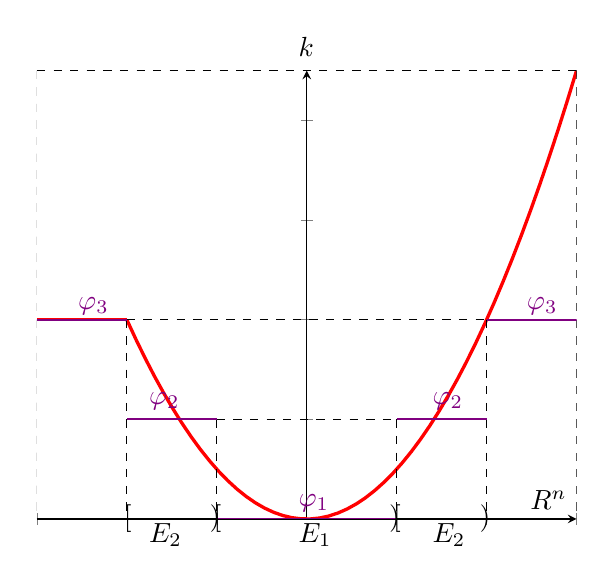
\begin{tikzpicture}
\begin{axis}[
axis y line=middle,
axis x line=middle,
xlabel=$\mathbb{R}^n$,
%grid = both, %major/minor
xticklabels={},yticklabels={}
];
\addplot [
very thick,red,mark=none,
domain=-2:3,samples=50,
] {(x^2)};
\addplot [
very thick,red,mark=none,
domain=-3:-2,samples=50,
] {4};
\draw [dashed] (-1,2) -- (1,2);
\draw [dashed] (-2,4) -- (2,4);
\draw [dashed] (-3,9) -- (3,9);

 \draw [dashed] (-1,2) -- (-1,0);
 \draw [dashed] (1,2) -- (1,0);
\draw [dashed] (-2,4) -- (-2,0);
\draw [dashed] (-3,9) -- (-3,0);
\draw [dashed] (2,4) -- (2,0);
\draw [dashed] (3,9) -- (3,0);

\draw[violet,  thick] (-1,0) -- (1,0);
\draw[violet,  thick] (-1,2) -- (-2,2);
\draw[violet,  thick] (1,2) -- (2,2);
\draw[violet,  thick] (2,4) -- (3,4);
\draw[violet,  thick] (-2,4) -- (-3,4);
   
\end{axis}

\node[color=black,right] at (3.2,-0.2) {$E_1$};
\node[color=black,right] at (1.3,-0.2) {$E_2$};
\node[color=black,right] at (4.9,-0.2) {$E_2$};
\node[color=black,right] at (3.2,6) {$k$};

\node[color=black,right] at (2.12,0) {$[$};
\node[color=black,right] at (2.07,0) {$)$};
\node[color=black,right] at (0.98,0) {$[$};
\node[color=black,right] at (4.35,0) {$)$};
\node[color=black,right] at (4.4,0) {$[$};
\node[color=black,right] at (5.5,0) {$)$};

\node[color=violet,right] at (3.2,0.2) {$\varphi_1$};
\node[color=violet,right] at (1.3,1.5) {$\varphi_2$};
\node[color=violet,right] at (4.9,1.5) {$\varphi_2$};
\node[color=violet,right] at (0.4,2.7) {$\varphi_3$};
\node[color=violet,right] at (6.1,2.7) {$\varphi_3$};
\end{tikzpicture}$$
Fijado un entero $k> 0$, definimos los siguientes conjuntos:
$$E_j^k := f^{-1}\left([(j-1)\cdot 2^{-k}, j\cdot 2^{-k} )\right)$$
Con dicha definición, es sencillo ver que los conjuntos son medibles, disjuntos y su unión queda como
$$\bigcup_{j=1}^{k\cdot 2^k}E_j^k = \{x\in  \mathbb{R}^n: f(x) < k\}$$
Definimos la siguiente función simple:
$$\varphi_k := \sum_{j=1}^{k\cdot 2^k} \frac{j-1}{2^k} \chi_{E_j^k}$$
Esto genera una sucesión de funciones creciente que denotamos por $\{\varphi_k\}_{k=1}^\infty \uparrow$.

Luego, por la definición que se ha dado de los $E_j^k$, dado $x \in \mathbb{R}^n,\ \exists k\in \mathbb{N} : \forall k \ge k_0: k > f\left(x\right) \Rightarrow x \in E_j^k$ para algún $j $ y, por tanto:
$$0 < f\left(x \right) - \varphi_k \left(x\right) < \frac{1}{2^k},\ \lim_{k \rightarrow \infty} \varphi_k\left(x\right) = f\left(x\right) $$
\end{demo}

\begin{prop}
Si $f, g: \mathbb{R}^n \rightarrow \mathbb{R}$ son funciones medibles no negativas, entonces la integral es aditiva, es decir:
$$\int_{\mathbb{R}^n} \left(f + g\right) \dif{\mu} = \int_{\mathbb{R}^n} f \dif{\mu} = \int_{\mathbb{R}^n} g \dif{\mu}$$
\end{prop}
\begin{demo}
Por la proposición anterior, existen dos sucesiones $\{\varphi_k\}_{k=1}^\infty$ y $\{\psi_k\}_{k=1}^\infty$ convergentes a $f$ y a $g$ respectivamente. De este modo, es trivial comprobar que $\{\varphi_k + \psi_k\}_{k=1}^\infty$ converge a $f+g$ y por el Teorema de Convergencia Monótona, tenemos que
$$\int_{\mathbb{R}^n}(f+g) \dif{\mu} = \lim_{k\rightarrow\infty} \int_{\mathbb{R}^n}(\varphi_k + \psi_k) \dif{\mu} = \lim_{k \rightarrow \infty} \left( \int_{\mathbb{R}^n} \varphi_k \dif{\mu} + \int_{\mathbb{R}^n} \psi \dif{\mu} \right) = \int_{\mathbb{R}^n} f \dif{\mu} + \int_{\mathbb{R}^n} g \dif{\mu}$$
\end{demo}

\begin{prop}
Sea $f: \mathbb{R}^n \rightarrow \mathbb{R}$ una función medible no negativa y $c\in \mathbb{R}^+$, entonces: 
$$\int_{\mathbb{R}^n} \left(c f\right) \dif{\mu} = c \int_{\mathbb{R}^n}f \dif{\mu}$$
\end{prop}
\begin{demo}
Completamente análoga a la anterior y se deja como ejercicio.
\end{demo}

\begin{theo}[Convergencia monótona para series]
Sea $\{f_k\}_{n=1}^{\infty}$ una sucesión de funciones medibles no negativas, entonces: 
$$\int_{\mathbb{R}^n} \left(\sum_{k=1}^{\infty} f_k \right) \dif{\mu} = \sum_{k=1}^{\infty}\left( \int_{\mathbb{R}^n} f_k \dif{\mu}\right)$$
\end{theo}
\begin{demo}
La demostración es prácticamente consecuencia de los enunciados anteriores:
$$\int_{\mathbb{R}^n} \left(\sum_{k=1}^{\infty} f_k\right) \dif{\mu} = \int_{\mathbb{R}^n} \lim_{m \rightarrow \infty} \left(\sum_{k=1}^{m} f_k \right)\dif{\mu} = \lim_{m \rightarrow \infty}\int_{\mathbb{R}^n} \left(\sum_{k=1}^{m} f_k\right) \dif{\mu} = $$
$$=\lim_{m \rightarrow \infty} \sum_{k=1}^{m} \left(\int_{\mathbb{R}^n} f_k \dif{\mu}\right) = \sum_{k=1}^{\infty} \left(\int_{\mathbb{R}^n} f_k \dif{\mu}\right) $$
\end{demo}

\begin{lema}[de Fatou]
Sea $\{f_k\}_{k=1}^{\infty}$ una sucesión de funciones medibles no negativas, entonces: 
$$\int_{\mathbb{R}^n} \left( \liminf_{k \rightarrow \infty}f_k \right) \dif{\mu} \le \liminf_{k \rightarrow \infty} \left(\int_{\mathbb{R}^n} f_k \dif{\mu}\right) $$
\end{lema}
\begin{demo}
Definimos las funciones $g_k = \inf_{m \ge k} f_m \ge 0$ medibles de modo que estas forman una sucesión creciente $\{g_k\}_{k=1}^\infty\uparrow$. En consecuencia, basta ver que:
$$\int_{\mathbb{R}^n} \left(\liminf_{k \rightarrow \infty}f_k \right) \dif{\mu} = \int_{\mathbb{R}^n} \left(\lim_{k \rightarrow \infty}g_k \right)\dif{\mu} =  \lim_{k \rightarrow \infty} \int_{\mathbb{R}^n} g_k \dif{\mu} = \liminf_{k \rightarrow \infty}\int_{\mathbb{R}^n} g_k \dif{\mu} \le \liminf_{k \rightarrow \infty} \int_{\mathbb{R}^n} f_k \dif{\mu}$$
\end{demo}

\begin{prop}
Las integrales impropias se soportan por la integral de Lebesgue:
\begin{align*}
\int_a^\infty f(x) \dif{x} = \int_{[a, \infty)}f(x)\dif{\mu} & &\int_a^b f(x)\dif{x} = \int_{[a,b]} f(x) \dif{\mu}
\end{align*}
\end{prop}
\begin{demo}
\begin{itemize}
\item Primera
$$\int_a^{\infty} f \left(x\right) dx = \lim_{M \rightarrow \infty} \int_a^M f \left(x\right) dx = \lim_{m \rightarrow \infty} \int_a^{\infty} f \left(x\right) \chi_{\left[a, M\right]}dx = \lim_{m \rightarrow \infty} \int_{\left[a, +\infty\right]} f \chi_{\left[a, M\right]} d \mu =$$
$$= \int_{\left[a, +\infty\right]} f \chi_{\left[a, +\infty\right]} d \mu = \int_{\left[a, +\infty\right]} f d \mu. $$
\item Segunda
$$\int_a^b f \left(x\right) dx = \lim_{k \rightarrow \infty}\int_a^{b - \frac{1}{k}} f \left(x\right) dx = \lim_{k \rightarrow \infty} \int_{\left[a, b - \frac{1}{k}\right]} f d \mu =$$
$$= \lim_{k \rightarrow \infty} \int_{\mathbb{R}} f \chi_{\left[a, b - \frac{1}{k}\right]} d \mu = \int_{\mathbb{R}} f \chi_{\left[a, b\right]} d \mu = \int_{\left[a, b\right]} f d \mu.$$
\end{itemize}
\end{demo}

\section{Funciones Integrables}
Hasta ahora no hemos hecho más que definir la integral y las propiedades que tiene y todo ello mayoritariamente para funciones no negativas. En esta sección, el objetivo es ampliar las miras y dar una definición consistente con las propiedades ya vistas para funciones no negativas y así poder sacarle completamente partido al concepto de integral.

\begin{defi}
Sea $f: \mathbb{R}^{n} \rightarrow \mathbb{R}$ una función medible\footnote{No necesariamente no negativa}, entonces diremos que es integrables si y sólo si: 
$$\int_{\mathbb{R}^n} \vert f \vert \dif{\mu} < +\infty$$
\end{defi}

\begin{obs}
Cabe destacar que dicha definición de integrabilidad para funciones no negativas tiene como consecuencia que puede haber funciones cuya integral en el sentido de Riemann converja (puesto que haya partes negativas que anulen partes positivas), pero que no sea integrable desde el punto de vista de Lebesgue.
\end{obs}

\begin{defi}
Dada una función medible $f: \mathbb{R}^{n} \rightarrow \mathbb{R}$, definimos:
\begin{align*}
f^+ := \max \{f, 0 \} & & f^- := -\min \{f, 0\}
\end{align*}

$$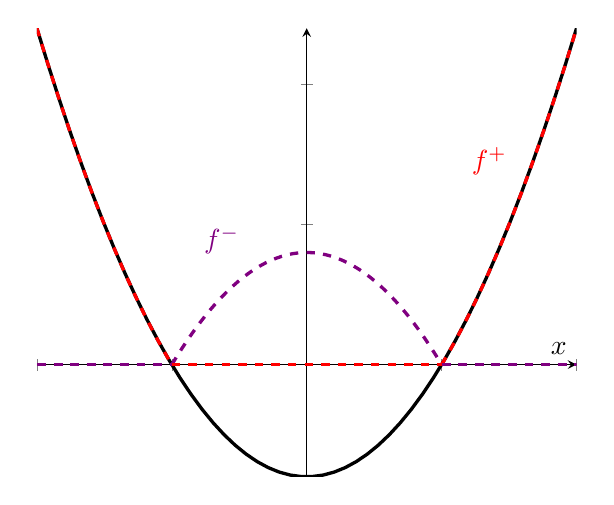
\begin{tikzpicture}
\begin{axis}[
axis y line=middle,
axis x line=middle,
xlabel=$x$,
%grid = both, %major/minor
xticklabels={},yticklabels={}
];

\addplot [
very thick,black,mark=none,
domain=-4:4,samples=50,
] {x^2 - 4)};

\addplot [
very thick,red,mark=none, dashed,
domain=-4:-2,samples=50,
] {x^2 - 4)};
\addplot [
very thick,red,mark=none, dashed,
domain=2:4,samples=50,
] {x^2 - 4)};
\addplot [
very thick,violet,mark=none,dashed,
domain=-2:2,samples=50,
] {abs(x^2 - 4))};

\addplot [
very thick,violet,mark=none,dashed,
domain=-4:-2,samples=50,
] {0};
\addplot [
very thick,violet,mark=none,dashed,
domain=2:4,samples=50,
] {0};

\addplot [
very thick,red,mark=none,dashed,
domain=-2:2,samples=50,
] {0};
\end{axis}
\node[color=red,right] at (5.4,4) {$f^+$};
\node[color=violet,right] at (2,3) {$f^-$};
\end{tikzpicture}$$

que verifican las siguientes propiedades:
\begin{enumerate}
\item $f^+ \; \land \; f^-$ son medibles y no negativas.
\item $f^+ - f^- = f$. 
\item $f^+ + f^- = \vert f \vert$
\item $f^+ \le \vert f \vert\; \land \;f^- \le \vert f \vert$ 
\end{enumerate}    
\end{defi}

\begin{prop}
Si $f: \mathbb{R}^n\rightarrow\mathbb{R}$ es una función integrable, entonces $f^+$ y $f^-$ son integrables, es decir:
\begin{align*}
\int_{\mathbb{R}^n} f^+ \dif{\mu} < +\infty & & \int_{\mathbb{R}^n} f^- d \mu < +\infty
\end{align*}
\end{prop}
\begin{demo}
Basta con ver que ambas funciones están acotadas por el módulo de $f$ y, por tanto, si $f$ es integrable, estas también lo son.
\end{demo}

En consecuencia, podemos dar una definición alternativa de la que se ha dado de función integrable que es completamente compatible e intercambiable con la que se ha dado anteriormente.

\begin{defi}
Sea $f: \mathbb{R}^{n} \rightarrow \mathbb{R}$ una función integrable, entonces podemos expresar su integral como: 
$$\int_{\mathbb{R}^n} f \dif{\mu} = \int_{\mathbb{R}^n} f^+ \dif{\mu} - \int_{\mathbb{R}^n} f^- \dif{\mu}$$
\end{defi}

\begin{obs}
Podríamos dar la misma definición de integrabilidad que se dió para funciones arbitrarias, pero ahora para funciones que toman valores en la recta ampliada. Sin embargo, cabe observar que $A=\{x\in \mathbb{R}: |f(x)|< \infty\}$ tiene que tener medida en caso de que dicha función sea integrable, puesto que:
$$\mu(A) > 0 \Rightarrow \forall k \in \mathbb{N}: k\cdot \chi_A \leq |f| \Rightarrow \int_{\mathbb{R}^n} |f| \ d\mu \geq I(k\chi_A) = k \cdot \mu(A)$$
Dicho de otra manera, siendo $B = \left\{ x : \lvert f\left( x \right) \rvert = + \infty \right\}$ tenemos que:
\[
m \left( B \right) = 0
\]
ya que tenemos que, $N \chi_A \left( x \right) \le \lvert f\left( x \right) \rvert \chi_A \left( x \right)$. Por tanto:
\[
\int N \chi_A \left( x \right) \mathrm{d}\mu \le \int \lvert f\left( x \right) \rvert \chi_A \left( x \right) \mathrm{d}\mu < \int \lvert f\left( x \right) \rvert \mathrm{d} \mu < +\infty
\]
que solo es posible si $\mu\left( A \right) = 0$.
\end{obs}

\begin{prop}
Supongamos que tenemos dos funciones $f,g: \mathbb{R}^n \rightarrow [-\infty, \infty]$ y tales que $f=g$ (c.t.p.), entonces tenemos que:
$$f \mbox{ integrable }\Leftrightarrow g \mbox{ integrable}$$
Y además las integrales coinciden:
$$\int_{\mathbb{R}^n} f \dif{\mu} = \int_{\mathbb{R}^n} g \dif{\mu}$$
\end{prop}
\begin{demo}
Como ya lo tenemos demostrado para funciones no negativas, basta con trabajar con las funciones $f^+$ y $f^-$, es decir:
$$f=g \ \mbox{c.t.p.}\Rightarrow \begin{cases}
f^+ = g^+ \\ f^- = g^- 
\end{cases} \mbox{c.t.p.}\Rightarrow \int f = \int f^+ - \int f^- = \int g^+ - \int g^- = \int g$$
\end{demo}

\begin{prop}
Son equivalentes:
\begin{itemize}
\item $f$ integrable
\item $|f|$ integrable
\item $f^+$ y $f^-$ integrables
\end{itemize}
\end{prop}
\begin{demo}
\begin{itemize}
\item $3)\rightarrow 1)$
$$\int |f| = \int f^+ + \int f^- < \infty \Rightarrow f \mbox{ integrable}$$
\end{itemize}
\end{demo}

\begin{lema}
Sea $f$ una función integrable, si $f = g - h$ con ambas funciones medibles, no negativas e integrables, entonces se verifica:
$$\int f \dif{\mu}= \int g \dif{\mu} - \int h \dif{\mu}$$
\end{lema}
\begin{demo}
Suponemos sin pérdida de generalidad que las funciones toman valores en $\bar{\mathbb{R}}$, puesto que más adelante se explica como generalizar dicho lema. De este modo, podemos expresar $f$ como:
$$f = f^+ - f^- = g-h\Rightarrow f^+ + h = f^- + g$$
Como todo son funciones no negativas e integrables, la integral de la suma es la suma de las integrales, por tanto:
$$\int f^+ + \int h = \int (f^+ + h) = \int (f^- + g)  = \int f^- + \int g \Rightarrow \int f^+ - \int f^- = \int g - \int h$$
\end{demo}

\begin{obs}
Este lema es válido para funciones que toman valores en $\bar{\mathbb{R}}$ porque el conjunto donde los valores no son reales es de medida nula. Por tanto, las funciones son iguales en c.t.p. a las funciones de la hipótesis y para esas la demostración es válida, luego para estas también.
\end{obs}

\begin{theo}[Operaciones de Integrabilidad]
Sean $f,g: \mathbb{R}^n \rightarrow \mathbb{R}$ dos funciones integrables, entonces la integral de la suma es:
$$\int (f+g) \dif{\mu} = \int f \dif{\mu} + \int g \dif{\mu}$$
Del mismo modo, para $\alpha \in \mathbb{R}$ la integral del producto por $\alpha$ es:
$$\int (\alpha \cdot f) \dif{\mu} = \alpha \int f \dif{\mu}$$
\end{theo}
\begin{demo}
Por la desigualdad triangular, $|f+g|\leq |f| + |g|$ y como ambas son funciones son no negativas, se les puede aplicar el lema:
$$\int |f+g| \leq \int |f| + \int |g| < \infty $$
De este modo, ya sabemos que al menos la suma es integrable, ahora veamos que la integral es justo la suma de las integrales. Para ello, expresamos la suma de la siguiente forma:
$$f+ g = f^+ - f^- + g^+ - g^- = (f^+ + g^+) - (f^- + g^-)$$
Como dichas funciones son  no negativas y son integrables, tenemos que
$$\int (f+g) = \int (f^+ + g^+) - \int (f^- + g^- ) = \int f^+ + \int g^+ - \int f^- -\int g^-  = \int f + \int g$$
Cabe observar que es necesario el lema para probar dicha demostración puesto que no se tiene en general la igualdad:
$$f^+ + g^+ = (f+g)^+$$
\end{demo}

\begin{theo}[De convergencia dominada]
Sea $\{f_k\}_{k=1}^{\infty}\rightarrow f$ una sucesión convergente c.t.p. a una función $f$, donde las funciones $f_k: \mathbb{R}^n \rightarrow \mathbb{R}$ son medibles y $g: \mathbb{R}^n \rightarrow \left[0, +\infty\right]$ una función integrable que acota a $f$ c.t.p., es decir, $\vert f_k \vert \le g$ c.t.p., entonces:
$$\int_{\mathbb{R}^n} f \dif{\mu} = \lim_{k \rightarrow \infty} \int_{\mathbb{R}^n} f_k \dif{\mu}$$
\end{theo}
\begin{demo}
Sabemos que $\vert f \vert \le g$ c.t.p, luego tenemos que:
$$\int_{\mathbb{R}^n} \vert f \vert \dif{\mu} \le \int_{\mathbb{R}^n} g \dif{\mu} < +\infty$$
Por lo que ya sabemos que al menos $f$ es integrable (y por la misma razón las $f_k$ son integrables).

Como $\vert f_k \vert \le g \Rightarrow g + f_k \ge 0$, de este modo formamos la sucesión de funciones $\{g + f_k\}_{k=1}^{\infty}$ a la que podemos aplicar el lema de Fatou: 
$$\int_{\mathbb{R}^n} f \dif{\mu} + \int_{\mathbb{R}^n} g \dif{\mu} = \int_{\mathbb{R}^n} \left(f + g\right) \dif{\mu} = \int_{\mathbb{R}^n} \lim_{k \rightarrow \infty} \left(f_k + g\right) \dif{\mu} =\int_{\mathbb{R}^n} \liminf_{k \rightarrow \infty} \left(f_k + g\right)  \dif{\mu} \leq$$
$$ \stackrel{\text{Fatou}}{\le} \liminf_{k \rightarrow \infty}\int_{\mathbb{R}^n} \left(f_k + g\right) \dif{\mu} = \liminf_{k \rightarrow \infty} \left( \int_{\mathbb{R}^n} f_k \dif{\mu} + \int_{\mathbb{R}^n} g \dif{\mu} \right) = \left(\liminf_{k \rightarrow \infty} \int_{\mathbb{R}^n} f_k \dif{\mu}  \right) + \int_{\mathbb{R}^n} g \dif{\mu}$$
Luego ya tenemos la desigualdad
$$\boxed{\int_{\mathbb{R}^n} f \dif{\mu} \le \liminf_{k \rightarrow \infty}\left( \int_{\mathbb{R}^n} f_k \dif{\mu}\right)}$$
De forma análoga, tomamos la sucesión $\{-f_k + g\}_{k=1}^{\infty}$ y entonces:
$$\int_{\mathbb{R}^n} \left(-f\right) \dif{\mu} \le \liminf_{k \rightarrow \infty} \int_{\mathbb{R}^n} \left(-f_k\right) \dif{\mu} \Rightarrow - \int_{\mathbb{R}^n} f \dif{\mu} \le \liminf_{k \rightarrow \infty} \left(-\int_{\mathbb{R}^n} f_k \dif{\mu} \right) =$$
$$= -\limsup_{k \rightarrow \infty} \left(\int_{\mathbb{R}^n} f_k \dif{\mu} \right) \Rightarrow \boxed{\limsup_{k \rightarrow \infty} \int_{\mathbb{R}^n} f_k \dif{\mu} \le \int_{\mathbb{R}^n} f \dif{\mu}} $$
Como por la convergencia, se tiene que el límite superior e inferior coinciden con el límite global, se tiene la igualdad.
\end{demo}

%TODO: Antes de esta sección por el libro. 3.2 y el 3.4
\subsection{Cálculo de integrales en \texorpdfstring{$\mathbb{R}^n$}{Rn}}
A pesar de que hemos definido todos los conceptos relativos al cálculo de integrales en $\mathbb{R}^n$, hasta ahora no hemos visto ningún método efectivo en términos prácticos para calcular integrales superiores a una dimensión. Aquí se desarrolla el Teorema fundamental que nos permite simplificar el cálculo de integrales en $\mathbb{R}^n$ al cálculo de varias integrales en $\mathbb{R}$.

\begin{defi}[Secciones de conjuntos]
Si tenemos un conjunto $A \subset \mathbb{R}^n \times \mathbb{R}^m$, podemos definir su \textbf{sección} como:
$$A_x = \{y \in \mathbb{R}^m: \left(x, y\right) \in A\}$$
\end{defi}
\begin{prop}[Principio de Cavalieri]
Sea $A \subset \mathbb{R}^n \times \mathbb{R}^m$ medible, entonces: 
\begin{enumerate}
    \item Los $A_x$ son medibles c.t.p $x\in \mathbb{R}^n$.
    \item La función $F: \mathbb{R}^n \rightarrow \left[0, +\infty\right]$ es medible y se define como:
    $$F \left(x\right) = \mu_m \left(A_x\right)$$
    \item $\mu_{n+m} \left(A\right) = \int_{\mathbb{R}^n} \mu_m \left(A_x\right) \dif{\mu_n} $
\end{enumerate}
\end{prop}
\begin{demo}
Junto al teorema de Tonelli.
\end{demo}

$$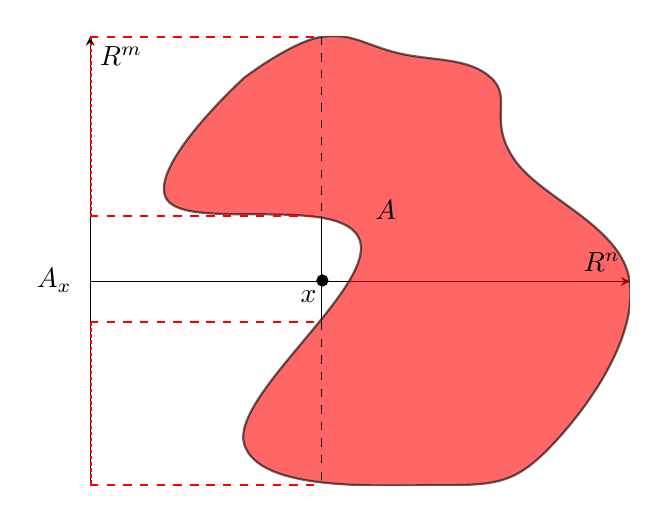
\begin{tikzpicture}
\begin{axis}[
tick style={draw=none},
axis y line=middle,
axis x line=middle,
xlabel=$\mathbb{R}^n$,
ylabel=$\mathbb{R}^m$,
xticklabels={},yticklabels={}
%grid = both, %major/minor
];
\addplot [thick, domain=0:7,fill=red, opacity=0.6]  plot[smooth, tension=.7] coordinates {(2,2.5) (3,3) (4,2.8) (5.2,2.5) (5.5,1.5) (7,0) (6,-2)(4.5,-2.5) (2,-2) (3.5,0.5) (1,1) (2,2.5)};

\draw [dashed] (3,3) -- (3,0.8);
\draw [solid] (3,0.8) -- (3,-0.5);
\draw [dashed] (3,-0.5) -- (3,-3);

\draw [densely dotted, very thick, red] (0,3) -- (0,0.8);
\draw [densely dotted, very thick, red] (0,-0.5) -- (0,-2.5);

\addplot [domain=0:3, samples=100, thick, color=red, dashed]{3};
\addplot [domain=0:3, samples=100, thick, color=red, dashed]{0.8};
\addplot [domain=0:3, samples=100, thick, color=red, dashed]{-0.5};
\addplot [domain=0:3, samples=100, thick, color=red, dashed]{-2.5};       
   

\end{axis}
\filldraw [black] (2.95,2.6) circle (2pt);
\node[color=black,right] at (-0.8,2.6) {$A_x$};
\node[color=black,right] at (2.55,2.4)  {$x$};
\node[color=black,right] at (3.5,3.5) {$A$};
\end{tikzpicture}$$

\begin{obs}
Si $N \subset \mathbb{R}^{n+m}$ satisface que $\mu_{n+m} \left(N \right) = 0$ hemos visto que para casi todo $x \in \mathbb{R}$ la sección $N_x$ es medible porque tiene medida nula. Sin embargo, puede ocurrir que para algún $x \in \mathbb{R}^n$ la sección $N_x$ no sea medible en $\mathbb{R}^m$

Por ejemplo, sea $E \subset \mathbb{R}$ no medible y sea $N = \{0\} \times E \subset \mathbb{R}^2$. Como $N$ está contenido en la recta $\{0\} \times \mathbb{R}$ está claro que $\mu_2 \left(N\right) = 0$, pero la sección $N_0 = E$ no es medible.
\end{obs}

\begin{coro}
Si la medida del conjunto es nula, entonces la medida de casi todas las secciones también lo es.
$$\mu_{n + m} \left(A\right) = 0 \Rightarrow \mu_m \left(A_x\right) = 0 \text{ c.t.p } x$$
\end{coro}

\begin{defi}[Secciones de funciones]
Sea $f: \mathbb{R}^{n} \times \mathbb{R}^n \rightarrow \mathbb{R}$ una función que expresaremos como $f \left(x, y\right)$ donde $x \in \mathbb{R}^n$ e $y \in \mathbb{R}^n$, llamamos \textbf{secciones} de $f$ a:
$$\forall x \in \mathbb{R}^n, \ f_x: \mathbb{R}^n \rightarrow \mathbb{R} \mbox{ donde } f_x \left(y\right) = f \left(x, y\right)$$
\end{defi}

\begin{lema}
Si $f$ y $g$ verifican el Tª de Tonelli y $a, b \in \mathbb{R}^+$, entonces la composición lineal de las funciones también, es decir, $af + bg$ cumple el Tª de Tonelli.
\end{lema}
\begin{demo}
Se ha de demostrar que en primer lugar, se tiene que:
$$\left(af + bg\right)_x = af_x + bg_x$$
Esta combinación lineal será medible, por serlo de funciones medibles y, por tanto:
$$F_{af + bg} = aF_f + bF_g$$ 
\end{demo}

\begin{lema}
Si una sucesión de funciones $\{f_k\}_{k=1}^{\infty}$ convergente puntualmente a $f$ cumple el Tª de Tonelli, entonces $f$ cumple el Tª Tonelli. 
\end{lema}
\begin{demo}
\begin{enumerate}
    \item Primero, vemos que
    $$f_x = \lim_{k \rightarrow \infty} \left(f_k\right)_x,\ \left(f_k\right)_x \uparrow f_x $$
    que es medible por ser límite de medibles
    \item En segundo lugar, como: 
    $$F = \lim_{k \rightarrow \infty}F_k,\ \{F_k\}_{k=1}^{\infty} \uparrow F \Rightarrow\lim_{k \rightarrow \infty} \int_{\mathbb{R}^m} \left(f_k\right)_x \dif{\mu} = \int_{\mathbb{R}^m} f_x \dif{\mu} $$
    \item Por último, tenemos que: 
    $$\int_{\mathbb{R}^n} F \dif{\mu} = \int_{\mathbb{R}^n} \lim_{k \rightarrow \infty}F_k  \dif{\mu} = \lim_{k \rightarrow \infty}\int_{\mathbb{R}^n} F_k \dif{\mu} = \lim_{k \rightarrow \infty} \int_{\mathbb{R}^n \times \mathbb{R}^m} f_k  \dif{\mu} = \int_{\mathbb{R}^n} f \dif{\mu}  $$
\end{enumerate}
\end{demo}

Como consecuencia de estos lemas el principio de Cavalieri es equivalente al teorema de Tonelli, es decir, basta con probar este principio para probar el teorema de Tonelli.

\begin{theo}[de Tonelli]
Sea $f: \mathbb{R}^{n} \times \mathbb{R}^m \rightarrow \left[0, +\infty\right)$ una función medible, entonces: 
\begin{enumerate}
    \item Para casi todo $x \in \mathbb{R}^n$, $f_x$ es medible en $\mathbb{R}^n$ (y no negativa).
    \item La función $F: \mathbb{R}^{n} \rightarrow \left[0, +\infty\right]$ es medible, donde se define como:
        $$F \left(x\right) = \int_{\mathbb{R}^m} f_x \dif{\mu_m} $$
    \item Se puede dividir la integral en secciones, es decir:
        $$\int_{\mathbb{R}^n \times \mathbb{R}^m} f \ \dif{\mu_{nm}} = \int_{\mathbb{R}^n} F \dif{\mu_n} $$
    expresado de forma más intuitiva:
    $$\int_{\mathbb{R}^n \times \mathbb{R}^m} f \left(x, y\right) \dif{x}\dif{y} = \int_{\mathbb{R}^n}\left(\int_{\mathbb{R}^m} f \left(x, y\right) \dif{y} \right)\dif{x} = \int_{\mathbb{R}^m}\left(\int_{\mathbb{R}^n} f \left(x, y\right) \dif{x} \right)\dif{y}$$
\end{enumerate}
Este teorema se podría enunciar de forma análoga para $y$, siendo entonces las hipótesis:
\begin{enumerate}
\item Para casi todo $y \in \mathbb{R}^m$, $f_y$ es medible en $\mathbb{R}^m$ (y no negativa).
\item La función $G: \mathbb{R}^n \rightarrow \left[0, \infty\right]$ es medible, donde se define como:
$$G \left(x\right) = \int_{\mathbb{R}^n} f_x \dif{\mu}$$
\item Se puede dividir la integral en secciones, es decir:
$$\int_{\mathbb{R}^n \times \mathbb{R}^m} f \dif{\mu} = \int_{\mathbb{R}^m} G \dif{\mu},$$
expresado de forma más intuitiva:
$$\int_{\mathbb{R}^n \times \mathbb{R}^m} f \left(x, y\right) \dif{x}\dif{y} = \int_{\mathbb{R}^m} \left(\int_{\mathbb{R}^n} f \left(x, y\right) \dif{x} \right) \dif{y}.$$
\end{enumerate}
\end{theo}
\begin{demo}
Para demostrar este teorema para funciones no negativas se irá demostrando para funciones más sencillas e incrementaremos la complejidad de forma gradual hasta llegar a las de las hipótesis.

\begin{enumerate}
\item Primeramente consideramos $f = \chi_{Q}$ donde $Q \subset \mathbb{R}^{n+m}$ es un cubo semiabierto, es decir, $Q = \prod_{i=1}^{n+m} \left[a_i, b_i\right)$. Este cubo se puede expresar en términos de otros dos, esto es, $Q = A \times B$ con $A \subset \mathbb{R}^n$ y $B \in \mathbb{R}^m$ cubos semiabiertos. Veamos entonces que:
\begin{enumerate}
    \item
    $$\left(\chi_Q\right)_x = \chi_{Q_x} = \begin{cases} \chi_B &  x \in A\\ 0 &  x \not\in A \end{cases} \Rightarrow \left(\chi_Q\right)_x$$
    $$\text{ ya que }Q_x = \begin{cases} B & x\in A \\ \emptyset & x\notin A \end{cases}\Rightarrow \chi_{Q_x} \text{ medible }\forall x \in \mathbb{R}^n$$
    \item
    $$F \left(x\right) = \int_{\mathbb{R}^m} \chi_{Q_x} \dif{\mu_m} = \begin{cases} \int_{\mathbb{R}^m} \chi_b \dif{\mu_m} = \mu_m \left(B\right) & x \in A \\ 0 & x \not\in A\end{cases} \text{ medible} \Rightarrow$$
    $$F \left(x\right) = \mu_m \left(B\right)\cdot \chi_A \left(x\right)$$
    \item
    $$\int_{\mathbb{R}^n} F \left(x\right) \dif{\mu_n} = \mu_m \left(B\right) \cdot \mu_n \left(A\right) = \mu_{n+m} \left(Q\right) = \int_{\mathbb{R}^n \times \mathbb{R}^m} \chi_Q \dif{\mu_{m+n}} $$
    Siendo la 2 igualdad cierta por tratarse de un cubo.
\end{enumerate}
\item Consideramos ahora $f = \chi_G$ donde $G \subset \mathbb{R}^{n+m}$ es un abierto. Por serlo, podemos escribirlo como $G = \bigsqcup_{j=1}^{\infty} Q_j$ donde cada $Q_j$ es un cubo semiabierto y la unión es disjunta.

Denotando $G_k = \bigsqcup_{j=1}^{k} Q_j$ tenemos que $\chi_{G_k} = \sum_{j=1}^{k} \chi_{Q_j}$. Por ser dicha función característica suma finita de funciones características de cubos (que ya sabemos que cumplen el Teorema), también cumple el Teorema por el primer lema y además vemos que $\{\chi_{Q_k}\}_{k=1}^{\infty} \uparrow \chi_G$ puntualmente, luego:
$$\chi_G = \sum_{j=1}^{\infty} \chi_{G_j} = \lim_{k \rightarrow \infty}\chi_{G_k} $$
De este modo, basta con aplicar el segundo lema y cumple el Teorema.

\item Supongamos que $f = \chi_D$ donde $D \subset \mathbb{R}^{n + m}$ es un conjunto $G_\delta$. En este caso, es suficiente considerar que $D$ es acotado puesto que $D$ se puede expresar como una unión creciente $$D = \bigcup_{k=1}^{\infty} D_k$$ donde cada $D_k$ es un $G_\delta$ y acotado (por ejemplo, $D_k = D \cap \left(-k, k\right)^{n+m}$). De este modo, $\{\chi_{D_k}\}_{k=1}^{\infty} \uparrow \chi_D$ y usando el segundo lema, ya lo tendríamos.

En consecuencia, supongamos que $D$ es $G_\delta $ y acotado, entonces escribimos
$$D = \bigcap_{k = 1}^{\infty} G_k$$
donde cada $G_k$ es abierto acotado y $G_1 \supset G_2 \supset G_k \supset \ldots \supset D$. De este modo, construimos la sucesión $\{\chi_{G_k}\}_{k=1}^{\infty} \downarrow \chi_D$ con la que, usando la versión decreciente de TCM, se puede hacer una demostración análoga a la del segundo lema para obtener que $\chi_D$ verifica el teorema. 

Alternativamente, como $0 \le \chi_D \le \chi_{G_1}$ es integrable y satisface el teorema, entonces se puede aplicar el TCD.

\item Consideramos ahora $f = \chi_N$ donde $\mu_{n+m} \left(N\right) = 0$. Por la regularidad de la medida, tenemos que:
$$\forall k \in \mathbb{N},\ \exists G_k \subset \mathbb{R}^{n+m} \mbox{ abierto con } N \subset G_k  \mbox{ y }  \mu_{n+m} \left(G_k \setminus N\right) < \frac{1}{k}$$

Si definimos $G:= \bigcap_{k \in \mathbb{N}} G_k$, entonces vemos que $G$ es un $G_\delta$ por ser intersección numerable de abiertos, tal que $N \subset G $ y además: 
$$\mu_{n+m} \left(G\setminus N\right) \le \forall k \in \mathbb{N}: \mu_{n+m} \left(G_k \setminus N\right) < \frac{1}{k} \xrightarrow{k\rightarrow \infty} 0 \Rightarrow \mu_{n+m}(G) = 0$$

De este modo, hemos encontrado un $G_\delta$ que contiene a $N$. En primer lugar, vemos que $\chi_G$ satisface el teorema para casi todo $x \in \mathbb{R}^n$ por el apartado anterior y, por tanto, $\chi_G$ es medible, luego:
$$0 = \mu_{n+m} \left(G\right) = \int_{\mathbb{R}^n \times \mathbb{R}^m} \chi_{G} \dif{\mu_{n+m}} = \int_{\mathbb{R}^n} \left( \int_{\mathbb{R}^m} \chi_{G_x}  \dif{\mu_m} \right) \dif{\mu_n}.$$
Por tanto, como la integral de dentro es la $F(x)$ del enunciado y es positiva:
$$\mu_m \left(G_k\right) = \int_{\mathbb{R}^m} \chi_{G_x} \dif{\mu_m} = 0 \text{ en casi todo punto } x \in \mathbb{R}^n$$
Como $N_x \subset G_x\Rightarrow \mu_m(N_x) \leq \mu_m(G_x) = 0 \Rightarrow \mu_m(N_x) = 0$ y además es medible, luego tenemos que $\chi_{N_x} = \left(\chi_N\right)_x = f_x$ es medible en para c.t.p. de $\mathbb{R}^n$.

Para la segunda consecuencia basta ver que:
$$0 \le F \left(x\right) = \int_{\mathbb{R}^m} \chi_{N_x} \dif{\mu_m} \le \int_{\mathbb{R}^m} \chi_{G_x} \dif{\mu_m} = 0 \text{ c.t.p. } \in \mathbb{R}^n$$
Por lo que, en particular, $F$ es medible.

Y, por último, hay que ver que la integral se puede iterar:
$$\int_{\mathbb{R}^n \times \mathbb{R}^m} \chi_N \dif{\mu_{n+m}} = 0 = \int_{\mathbb{R}^n} \underbrace{F \left(x\right)}_{=0} \dif{\mu_n} = \int_{\mathbb{R}^n} \left(\int_{\mathbb{R}^m} \chi_{N_x} \dif{\mu_m} \right) \dif{\mu_n} $$

\item Sea ahora $f = \chi_A$ donde $A \subset \mathbb{R}^{n+m}$ es medible. Por ser medible, sabemos que podemos descomponer $A$ como $A = D \setminus N$, donde $D$ es un $G_\delta $ y $\mu_{n+m} \left(N\right) = 0$. Por tanto, $D = A \sqcup N \Rightarrow \chi_D = \chi_A + \chi_N$ y, en consecuencia:
$$\chi_A = \chi_D - \chi_N \text{ para c.t.p. } x \in \mathbb{R}^n$$
Y es sencillo ver que también se cumple la igualdad:
$$\chi_{A_x}= \chi_{B_x} - \chi_{N_x} \text{ es medible por (3) y (4)}$$

Para ver la segunda conclusión, tenemos que: 
$$F \left(x\right) = \int_{\mathbb{R}^m} \chi_{A_x} \dif{\mu_m} = \int_{\mathbb{R}^m} \chi_{D_x} \dif{\mu_m}$$
puesto que $\mu_m \left(N_x\right) = 0$ y entonces es medible para c.t.p. $x \in \mathbb{R}^n$ porque $D$ es $G_\delta$ y aplicamos el apartado (3).

Para terminar:
$$\int_{\mathbb{R}^n} F \left(x\right) \dif{\mu_n} = \int_{\mathbb{R}^n} \left( \int_{\mathbb{R}^m} \chi_{A_x} \dif{\mu_m} \right) \dif{\mu_n} = \int_{\mathbb{R}^n} \left(\int_{\mathbb{R}^m} \chi_{D_x} \dif{\mu_m} \right) \dif{\mu_n} = $$
$$= \int_{\mathbb{R}^n \times \mathbb{R}^m} \chi_{D} \dif{\mu_{n+m}} = \mu_{n+m} \left(D\right) = \mu_{n+m} \left(A\right) = \int_{\mathbb{R}^n \times \mathbb{R}^m} \chi_A \dif{\mu_{n+m}} $$
Porque $D_x$ si verificaba ya el Teorema de Tonelli.

\item Sea $f$ función simple, medible, no negativa, entonces $f$ es combinación lineal no negativa de funciones características de conjuntos medibles en $\mathbb{R}^n \times \mathbb{R}^m$ y por el lema trivialmente se tiene.

\item Finalmente, consideramos $f$ medible no negativa. Como para estas funciones hemos demostrado que $ \exists \{f_k\}_{k=1}^{\infty}\uparrow f$ donde cada $f_k$ es simple, medible y no negativa, queda probado por el lema 2 y el apartado 6.
\end{enumerate} 
\end{demo}

\begin{ej} 
Si $A \subset \mathbb{R}^n \times \mathbb{R}^m$:
$$\int_A f \left(x, y\right) \dif{x} \dif{y} = \int_{\mathbb{R}^n \times \mathbb{R}^m} f \left(x, y\right) \chi_A \left(x, y\right) \dif{x}\dif{y} = $$
$$\int_{\mathbb{R}^n} \left(\int_{\mathbb{R}^m} f \left(x, y\right) \chi_A \left(y\right) \dif{y} \right) \dif{x} = \int_{\mathbb{R}^n} \left(\int_{A_x} f \left(x, y\right) \dif{y}\right) \dif{x}$$
\end{ej}

\begin{theo}[de Fubini]
Sea $f: \mathbb{R}^n \times \mathbb{R}^m \rightarrow \mathbb{R}$ integrable. Entonces: 
\begin{enumerate}
\item Para c.t.p. $x \in \mathbb{R}^n$, $f_x$ es integrable en $\mathbb{R}^n$.
\item La función $F: \mathbb{R}^n \rightarrow \left[0, \infty\right]$ es medible en $\mathbb{R}^n$, donde $F$ está definida en c.t.p. como:
$$F \left(x\right) = \int_{\mathbb{R}^m} f_x \dif{\mu}_m$$

\item Se puede dividir la integral en secciones, es decir:
$$\int_{\mathbb{R}^n \times \mathbb{R}^m} f \dif{\mu}_{n+m} = \int_{\mathbb{R}^n} F \dif{\mu}_n,$$
\end{enumerate}
\end{theo}
\begin{demo}
\begin{enumerate}
Podemos escribir $f = f^+ - f^-$. De nuevo, es sencillo ver que $\forall x \in \mathbb{R}^n : \left(f^+\right)_x = \left(f_x\right)^+ \; \land \; \left(f^-\right)_x = \left(f_x\right)^-$, por tanto como $f^+$ y $f^-$ verifican el teorema de Tonelli, entonces $f^+_x $ y $f^-_x$ son medibles c.t.p $x \in \mathbb{R}^n$ y como $f_x = \left(f^+_x\right) - \left(f^-_x\right)$ también es medible c.t.p $x \in \mathbb{R}^n$.

Tanto la $f^+$ como la $f^-$ son integrales porque:
 $$\int_{\mathbb{R}^n} \left(\int_{\mathbb{R}^m} f^+_x \dif{\mu_m} \right) \dif{\mu_n} = \int_{\mathbb{R}^n \times \mathbb{R}^m} f^+ \dif{\mu_{n+m}} < \infty$$
Por tanto, $F \left(x\right) = \int_{\mathbb{R}^n} f^+_x \dif{\mu_n} + \int_{\mathbb{R}^n} f^-_x \dif{\mu_n}$ es finita en c.t.p., luego integrable.
\end{enumerate}
\end{demo}

\begin{obs}
El problema, en general, es demostrar que una función es integrable para poder aplicar este teorema. Un método útil suele ser demostrar que $\int_{\mathbb{R}^n} \left(\int_{\mathbb{R}^m} \vert f \left(x, y\right) \vert \dif{y} \right) \dif{x} < \infty$ y como con el valor absoluto es no negativa podemos aplicar Tonelli a $\vert f\vert$ y separar la integral para demostrar que $f$ es integrable.
\end{obs}

\begin{ej}
Consideramos $E = \{ \left(x, y\right) \in \mathbb{R}^2 : 0 \leq x \leq y\}$ y $f \left(x, y\right) = e^{-y^2}$ y vamos a ver que es integrable en $E$ y a calcular su integral:
\begin{itemize}
    \item En primer lugar, $f \left(x, y\right) = e^{-y^2} \ge 0$ es medible por ser continua en $\mathbb{R}^2$.
    \item En segundo lugar, como es positiva por el Teorema de Tonelli es integrable y la integral se puede calcular como: 
    $$\int_E f \left(x, y\right) \dif{x} \dif{y} = \int_{\mathbb{R}^2} f \left(x, y\right) \cdot \chi_{E} \left(x, y\right) \dif{x} \dif{y} = \int_{-\infty}^{\infty} \int_{-\infty}^{\infty} e^{-y^2}\chi_E \left(x, y\right) \dif{x} \dif{y} =$$
    $$=\int_{0}^{\infty} \int_{0}^{y} e^{-y^2} \dif{x} \dif{y} = \frac{1}{2} \int_{0}^{\infty} 2ye^{-y^2} \dif{y} = \left[\frac{1}{2} \left(e^{-y^2}\right)\right]_{y=0}^{y=\infty} = \frac{1}{2} \left(1 - 0\right) =\frac{1}{2}$$
\end{itemize}
\end{ej}

\begin{prop}
Sea $f: \left[a, \infty\right) \rightarrow \left[0, +\infty\right)$ continua, entonces la integral impropia coincide con la impropia de Riemann
$$\int_{[a, +\infty)} f = \lim_{R \rightarrow \infty} \int_a^R f $$
Nótese que esto se refiere a funciones \textbf{positivas}.
\end{prop}
\begin{demo}
Sea $a \le \{b_k\}{k=1}^{\infty}\uparrow \infty$ y definimos $f_k = f \cdot \chi{\left[a, b_k\right]}$. Así, $\{f_k\}_{k=1}^{\infty}\uparrow f$ luego por el Teorema de la Convergencia Monótona
$$\int_{\left[a, \infty\right)} f = \lim_{k \rightarrow \infty} \int_{\left[a, \infty\right)} f_k = \lim_{k \rightarrow \infty} \int_a^{b_k} f $$
\end{demo}

\begin{ej}
Consideramos $A = \left[0, 1\right] \times \left[0, +\infty\right]$ y la función $f \left(x, y\right) = e^{-y} \sen \left(2xy\right)$ y vamos a demostrar que es integrable y a calcular la integral.
\end{ej}

\begin{itemize}
    \item En primer lugar, para poder aplicar el Teorema de Fubini, necesitamos ver que $f$ es integrable, es decir, $\int_A \vert f\vert < \infty$, luego calculamos:
    $$\vert f \left(x, y\right)\vert = \vert e^{-y} \sen \left(2xy\right)\vert \le e^{-y}$$
    $$\int_A \vert f \left(x, y\right) \vert \le \int_A e^{-y} \dif{x} \dif{y} = \int_0^1 \int_0^{\infty} e^{-y} \dif{y} \dif{x} = \left(\int_0^1 1 \dif{x}  \right) \left(\int_0^{\infty} e^{-y} \dif{y} \right) = 1 < \infty $$
\item Una vez que sabemos que es integrable, aplicamos Fubinni:
    $$\int_A f \left(x, y\right) \dif{x} \dif{y} = \int_0^1 \left(\underbrace{\int_0^{\infty} e^{-y}\sen\left(2xy\right) \dif{y}}_{F \left(x\right)} \right) \dif{x}  = **$$
    \begin{itemize}
    	\item Veamos primero la $F \left(x\right)$:
    $$\begin{cases}
        u = \sen \left(2xy\right) & du = 2x \cos \left(2xy\right)dy \\\\
        dv = e^{-y}dx & v = -e^{-y}
    \end{cases} \Rightarrow$$
    $$F \left(x\right) = \underbrace{\left[-e^{-y} \sen \left(x, y\right)\right]_{0}^{\infty}}_{= 0} + \int_0^{\infty} 2xe^{-y}\cos \left(2xy\right) \dif{y}$$
    $$\begin{cases}
        u = 2x\cos \left(2xy\right) & du = \left(2x\right)^2 \cdot \left(-\sen \left(2xy\right)\right)dy \\
        dv = e^{-y}dy & v = -e^{-y}
    \end{cases}$$
    $$F(x)=\left[-e^{-y}2x \cos \left(2xy\right)\right]_{0}^{\infty} - \int_0^{\infty} 4x^2e^{-y}\sen \left(2xy\right) \dif{y} = 2x - 4x^2 F \left(x\right)\Rightarrow$$
    $$\Rightarrow F \left(x\right) \cdot \left(1 + 4x^2\right) = 2x \Rightarrow F \left(x\right) = \frac{2x}{1+4x^2}$$
    	\item Volviendo a la integral original:
    $$\int_0^1 \frac{1}{4} \cdot \frac{8x}{1+4x^2} \dif{x} = \frac{1}{4} \left[\log \left(1 + 4x^2\right)\right]_{0}^{1} = \frac{\log \left(5\right)}{4}.$$
    \end{itemize}
\end{itemize}

\begin{prop}
Sea $f: \left[a, \infty\right) \rightarrow \mathbb{R}$ continua, si es integrable, entonces la integral impropia coincide con la impropia de Riemann:
$$\lim_{R \rightarrow \infty} \int_a^k f = \int_{\left[a, \infty\right)} f $$
Nótese que esto es cierto para funciones \textbf{con valores en $\mathbb{R}$}.
\end{prop}

\begin{demo}
Sea $a \le \{b_k\}{k=1}^{\infty}\uparrow \infty$ y sean $f_k = f \cdot \chi{\left[a, \infty\right)}$. Entonces, $ \{f_k\}k \rightarrow f$ puntualmente y además $\vert f_k \vert \le \vert f \vert \text{ ,que es integrable en } \left[a, \infty\right)$ Así, por el Teorema de la Convergencia Dominada, $$\lim{k \rightarrow \infty} \int_a^{b_k} f = \int_a^{\infty} f$$ 
\end{demo}

\begin{defi}[Funciones definidas por integrales]
Una función viene definida por una integral si tiene la siguiente forma: 
$$F \left(u\right) = \int_{\mathbb{R}^n} f \left(x, u\right) \dif{x} $$
Donde para un $u$ fijo, se integra la función sobre las componente $x$ libre y en su medida concreta.
\end{defi}

\begin{theo}
Sea $\mathcal{U} \subset \mathbb{R}^m$ y sea $f: \mathbb{R}^n \times \mathcal{U} \rightarrow \mathbb{R}$, supongamos que: 
\begin{enumerate}
    \item $\forall u \in \mathcal{U},\ f_{u}: \mathbb{R}^n \rightarrow \mathbb{R}$ es integrable.
    \item $\forall x \in \mathbb{R}^n,\ f_x: \mathcal{U} \rightarrow \mathbb{R}$ es continua.
    \item $\exists g: \mathbb{R}^n \rightarrow \mathbb{R}$ integrable tal que $\vert f \left(x, u\right) \vert \le g \left(x\right),\ \forall x \in \mathbb{R}^n,\ \forall u \in \mathcal{U}$
\end{enumerate}
Entonces se verifica la continuidad de la definida por la integral: 
$$F \left(u\right) = \int_{\mathbb{R}^n} f \left(x, u\right) \dif{x} \text{ es continua en } \mathcal{U}.$$
\end{theo}
\begin{demo}
Sea $\{u_k\}_{k=1}^{\infty} \subset \mathcal{U}$ con $u_k \rightarrow u_0$ en $\mathcal{U}$, definimos $\forall k \in \mathbb{N}: f_k = f{u_k} = f \left(x, u_k\right) \rightarrow f \left(x, u\right)$. Además, como se tiene que $\vert f_k \left(x\right) \vert = \vert f \left(x, u_k\right) \vert \le g \left(x\right)$ y esto para $\forall x \in \mathbb{R}^n$ y $\forall k \in \mathbb{N}$, por el TCM: 
$$\underbrace{\int_{\mathbb{R}^n} f_k \left(x\right) \dif{x}}_{F \left(u_k\right)} \rightarrow \underbrace{\int_{\mathbb{R}^n} f \left(x, u_0\right) \dif{x}}_{= F \left(u_0\right)} $$
\end{demo}

\begin{theo}[Regla de Leibniz]
Sea $f: \mathbb{R}^{n} \times \left[a, b\right] \rightarrow \mathbb{R}$ una función medible y $F \left(t\right) = \int_{\mathbb{R}^n} f \left(x, t\right) \dif{x}$ la definida por la integral de dicha función, supongamos que: 
\begin{enumerate}
    \item $\forall r \in \left[a, b\right],\ f_r: \mathbb{R}^{n} \rightarrow \mathbb{R}$ es integrable en $\mathbb{R}^n$.
    \item $\forall x \in \mathbb{R}^n : \ f_x: \left[a, b\right] \rightarrow \mathbb{R}$ es $C^{1)}$, donde $f_x \left(t\right) = f \left(x, t\right)$
    \item $\exists g: \mathbb{R}^n \rightarrow \mathbb{R}$ integrable tal que $\vert \frac{\partial f \left(x, t\right)}{\partial t}\vert \le g \left(x\right) : \forall x \in \mathbb{R}^n \mbox{ y }\forall k \in \left[a, b\right]$
\end{enumerate}
Entonces $F$ es $C^{1)}$ en $\left(a, b\right)$ y $\forall t \in \left(a, b\right)$ podemos definir su derivada: 
$$F' \left(t\right) = \int_{\mathbb{R}^n} \frac{\partial f \left(x, t\right)}{\partial t} \dif{x} $$
\end{theo}
\begin{demo}
Vamos a aplicar el Teorema de Fubini y de Tonelli a $\frac{\partial f\left(x, t\right)}{\partial t} $
\begin{itemize}
    \item En primer lugar, como podemos expresar dicha función como: 
    $$\frac{\partial f}{\partial t} \left(x, t\right) = \lim_{s \rightarrow 0^+} \frac{f \left(x, t + s\right) - f \left(x, t\right)}{s} = \lim_{k \rightarrow \infty} \frac{f \left(x, t + \frac{1}{k}\right) - f \left(x, t\right)}{\frac{1}{k}}$$
    es medible por ser límite puntual de funciones medibles.
    \item En segundo lugar, como podemos acotarla por una función integrable, es integrable en $\mathbb{R}^n \times \left[a, b\right]$:
    $$\int_{\mathbb{R}^n} \left\vert \frac{\partial f}{\partial t} \left(x, t\right)\right\vert  \dif{x} \dif{y} \le \int_{\mathbb{R}^n \times \left[a, b\right]} g \left(x\right) \dif{x} \dif{t} = \int_{\mathbb{R}^n} \left(\int_a^b g \left(x\right) \dif{t}  \right) \dif{x}  = $$
    $$ = \int_{\mathbb{R}^n} \left(b - a\right) g \left(x\right) \dif{x} = \left(b - a\right) \int_{\mathbb{R}^n} g(x) \dif{x}< +\infty$$
    \item Aplicamos el teorema de Fubini, es decir, $\forall s \in \left[a, b\right]$: 
    $$\int_a^s \left(\int_{\mathbb{R}^n} \frac{\partial f}{\partial t} \left(x, t\right) \dif{x} \right) \dif{t} = \int_{\mathbb{R}^n} \left(\int_a^s \frac{\partial f}{\partial t} \left(x, t\right) \dif{t} \right) \dif{x} = $$
    $$= \int_{\mathbb{R}^n} \left( f \left(x, s\right) - f \left(x, a\right)\right) \dif{x} = F \left(s\right) - F \left(a\right).$$
    Denotamos: 
    $$H \left(t\right) := \int_{\mathbb{R}^n} \frac{\partial f\left(x, t\right)}{\partial t}  \dif{x}$$
    Como $\frac{\partial f\left(x, t\right)}{\partial t}  = f_x' \left(t\right)$ es continua en $t$ y $\vert \frac{\partial f}{\partial t} \vert \le g$, por el Teorema anterior obtenemos que $H$ es continua en $t \in \left[a, b\right]$. En consecuencia, vemos que: 
    $$\int_a^s H \left(t\right) \dif{t} = F \left(s\right) - F \left(a\right) \Rightarrow F \left(s\right) = F \left(a\right) + \int_a^s H \left(t\right) \dif{t}$$
	Por el Teorema Fundamental del Cálculo:    
    $$F' \left(t\right) = H \left(t\right),\ \forall t \in \left(a, b\right) $$
\end{itemize}
\end{demo}

\begin{ej}
Supongamos la función 
$$F \left(t\right) = \int_0^{\infty} \frac{1 - e^{tx}}{xe^{x}} \dif{x} \text{\quad con } t > -1$$
En primer lugar, veamos que $F$ está bien definida y que es derivable en $t \in \left(-1, \infty\right)$:

Dado $t \in \left(-1, \infty\right)$ sean $-1 < a < t_0 < b <\infty$. Vamos a demostrar que $F$ es derivable $\left(C^1\right)$ en $\left(a, b\right)$. De aquí se deduce que $F$ es derivable $\left(C^1\right)$ en $\left(-1, \infty\right)$.

\begin{enumerate}
    \item En primer lugar, veamos que $\forall t > -1: f_t \left(x\right) = \frac{1 - e^{-tx}}{x} e^{-x}$ es una función integrable en $\left(0, \infty\right)$:
    $$\lim_{x \rightarrow 0^+} \frac{1 - e^{-tx}}{x} = \lim_{x \rightarrow 0^+} \frac{t\cdot e^{-tx}}{1} = t \in \mathbb{R}$$
    Luego $f_t$ se extiende con continuidad a x = 0, es decir, podemos tomar como $f_t(0)=t$ para que sea continua y la integral no cambia porque solo se diferencia en un punto con la función que realmente tenemos.
    
    Para ver que es integrable, tenemos que ver que su valor absoluto es integrable, es decir:
    $$\left\vert f_t \left(x\right)\right\vert = \left\vert \frac{1 - e^{-tx}}{x}\right\vert e^{-x} = \frac{\left\vert 1 - e^{-tx}\right\vert}{x} e^{-x}$$
    Si $x \geq 1$, entonces vemos que $\vert f_t \left(x\right) \vert \le \vert 1 - e^{-tx} e^{-x} \vert \le e^{-x} + e^{-\left(t+1\right)x}$, de este modo ya es sencillo ver que es integrable puesto que:
    \begin{align*}
    \int_1^{\infty} e^{-x} \dif{x} < \infty  && \int_1^{\infty} e^{-\left(t + 1\right)x} \dif{x} < \infty \text{ porque } t + 1 > 0
	\end{align*}

    \item En segundo lugar, vamos a ver que la derivada existe y es continua en $t$:
    $$\frac{\partial f\left(x, t\right)}{\partial t}  = \frac{xe^{-tx}}{x}e^{-x} = e^{-\left(t+1\right)x} \text{ existe y es continua en t}$$
    \item Por último, tenemos que ver dónde la parcial calculada es integrable:
    $$\left\vert \frac{\partial f}{\partial t} \left(x, t\right)\right\vert = e^{-\left(t+1\right)x}\stackrel{t=-1}{\Rightarrow} e^{-\left(t+1\right)x} = e^{0} = 1 \Rightarrow \text{ no integrable en } \left(0, \infty\right)$$

    Fijamos $-1 < a < b < \infty$ y consideramos el intervalo formado por ambos extremos $\left[a, b\right]$. Para un $t \in \left[a, b\right] \Rightarrow a \le t \Rightarrow e^{-\left(t+1\right)x} \le e^{-\left(a+1\right)x}$ que podemos tomar como $g \left(x\right)$ y vemos que:
    $$\int_0^{\infty} g \left(x\right) \dif{x} = \int_0^{\infty} e^{-\left(a+1\right)x} \dif{x} =  \left[\frac{e^{\left(a+1\right)x}}{a+1}\right]_{0}^{\infty} = \frac{1}{a+1} < \infty \text{ puesto que } a+1>0$$
    De este modo, $F$ derivable $C^{1)}$ en $\left(a, b\right)$ para cualesquiera $a,b \in (-1, \infty)$, por lo que $ F$ es $C^1$ en $ \left(-1, \infty\right)$.

    Además, podemos calcular la derivada $\forall t \in \left(a, b\right)\mbox{ y } \forall a, b : -1 < a < b < \infty$ como:
    $$F' \left(t\right) = \int_0^{\infty} \frac{\partial f\left(x, t\right)}{\partial t}  \dif{x} = \int_0^{\infty} e^{-\left(t + 1\right)} \dif{x} = \left[-\frac{e^{- \left(t + 1\right)x}}{t+1}\right]_{x = 0}^{x = \infty} = \frac{1}{t + 1}$$
    Por tanto, si escogemos $\forall t > -1$:
    $$F \left(t\right) = \int \frac{1}{1 + t} \dif{t} = \log \left(1 + t\right) + C$$
    Y para calcular el valor de la constante de integración basta con ver que:
    $$F \left(0\right) = \int_0^{\infty} 0 \dif{t} = 0 = \log \left(1\right) + C\Rightarrow C = 0$$
\end{enumerate}
\end{ej}

\section{Teorema del Cambio de Variable}
Del mismo modo que para poder integrar en $\mathbb{R}$ podíamos hacer cambios de variable que simplificasen las expresiones que se debía integrar, es posible definir un teorema equivalente para dimensiones superiores que nos permiten cambiar el sistema de coordenadas sobre el que describir los objetos matemáticos y seguir integrando cómodamente.

\begin{theo}
Sea $T: \mathbb{R}^n \rightarrow \mathbb{R}^n$ lineal, si $A \subset \mathbb{R}^n$ es medible, entonces $T \left( A\right)$ es medible y se tiene que:
$$\mu_n \left(T\left(A\right)\right) = \lvert det \left(T\right) \rvert \cdot \mu_n \left(A\right)$$
\end{theo}

\begin{obs}
En el caso en el que $det \left(T\right) = 0$, entonces $T$ no es sobreyectiva y, por tanto, $T \left(\mathbb{R}^n\right)$ es una espacio vectorial propio de $\mathbb{R}^n$, los cuales tienen $\mu_n \left(T \left(\mathbb{R}^n\right)\right) = 0$.
\end{obs}

\begin{defi}[Difeomorfismo]
Sea $U, V \subset \mathbb{R}^n$ abiertos, se dice que $\varphi: U \rightarrow V$ es un \textbf{difeomorfismo} si: 
\begin{enumerate}
    \item $\varphi: U \rightarrow V$ es $C^{1)}$.
    \item $\varphi: U \rightarrow V$ es biyectiva. 
    \item $\varphi^{-1}: V \rightarrow U$ es $C^{1)}$
\end{enumerate}
\end{defi}

\begin{obs}
Sea $U \subset \mathbb{R}^n$ abierto y $\varphi: U \rightarrow \mathbb{R}^n$ de clase $C'$ tal que $\varphi$ es inyectiva en $U$ y $det \left(J \varphi \left(u\right) \right) \neq 0,\ \forall u \in U \Rightarrow$ por el Teorema de la Función Inversa, sabemos que $V = \varphi \left(U\right)$ es abierto y su inversa $\varphi^{-1}: V \rightarrow U$ es $C^1$. Es decir, $\varphi U \rightarrow \varphi \left(U\right)$ es un difeomorfismo-$C^1$.
\end{obs}

\begin{theo}
Sea $\varphi: U \rightarrow V$ un difeomorfismo-$C^{1)}$ entre dos abiertos de $\mathbb{R}^n$, si $A \subset U$ es medible, entonces $\varphi \left(A\right)$ es medible y se tiene que:
$$\mu \left(\varphi \left(A\right) \right) = \int_A \lvert \det J \varphi\left(u\right) \rvert \dif{u}$$
\end{theo}

\begin{obs}
Este teorema es una generalización del anterior, puesto que si $\varphi = T: \mathbb{R}^n \rightarrow \mathbb{R}^n$ es un isomorfismo lineal, entonces recuperamos el enunciado anterior.
\end{obs}

\begin{theo}[Cambio de variable]
Sea $\varphi: U \rightarrow V$ un difeomorfismo-$C^{1)}$ donde $U, V\subset \mathbb{R}^n$ abiertos, si $A\subset U$ es medible y $f: V \rightarrow \mathbb{R}$ es integrable en $ \varphi \left(A\right)$, entonces $f \circ \varphi: U \rightarrow R$ es integrable en $A$ y la integral se expresa como:
$$\int_{\varphi \left(A\right)} f = \int_A f \circ \varphi \cdot \lvert \det J \varphi \rvert$$
Que si tomamos como $A= U$, sería
$$\int_V f = \int_U f \circ \varphi \cdot \lvert \det J \varphi \rvert$$
Si tratamos de ponerlo en una notación más habitual: 
$$\int_{\varphi \left(A\right)} f \left(x\right) \dif{x} = \int_A f \left(\varphi \left(u\right)\right) \cdot \lvert \det J \varphi \left(u\right) \rvert \dif{u}$$
\end{theo}

\begin{obs}
Este teorema es la generalización total de los dos anteriores, ya que si $f = \chi_{\varphi \left(A\right)}$ obtenemos el teorema anterior.
\end{obs}

\begin{ej}
Supongamos la siguiente integral $$\int_E e^{\frac{x - y}{x + y}} \dif{x} \dif{y}$$
definiendo $E$ como el triángulo de vértices: $\left(0, 0\right), \left(0, 2\right), \left(2, 0\right)$, es decir:
$$\begin{tikzpicture}
\begin{axis}[
axis y line=middle,
axis x line=middle,
%xlabel=$x$,
%grid = both, %major/minor
];

\addplot [domain=0:2, samples=100, name path=f, thick, color=red!50]
        {-x + 2};

\path [name path=xaxis]
      (\pgfkeysvalueof{/pgfplots/xmin},0) --
      (\pgfkeysvalueof{/pgfplots/xmax},0);

\addplot[red!10, opacity=0.4] fill between [of=f and xaxis, soft clip={domain=-2:2}];
\node[color=black,right] at (axis cs: 0,0.1) {$(0,0)$};
\node[color=black,right] at (axis cs: 0,1.9)  {$(0,2)$};
\node[color=black,right] at (axis cs: 1.7,0.1)  {$(2,0)$};
\node[color=black,right] at (axis cs: 0.5,0.7) {$E$};
\node[color=red, font=\footnotesize] at (axis cs: 1.3,1) {$x + y = 2$};
\end{axis}
\filldraw [black] (0,0) circle (2pt);
\filldraw [black] (6.8,0) circle (2pt);
\filldraw [black] (0,5.7) circle (2pt);
\end{tikzpicture}$$
Si tenemos por ejemplo, la transformación $\varphi^{-1} = \begin{cases} u = x - y\\ v = x + y 
\end{cases} \Rightarrow \varphi = \begin{cases} x = \frac{u + v}{2}\\ y = \frac{v - u}{2} \end{cases}$, entonces podemos ver que:
\begin{align*}
\varphi^{-1} \left(x + y = 2\right) \equiv v = 2 & & \varphi^{-1} \left(y = 0\right)\equiv u = v & & \varphi^{-1} \left(x = 0\right)\equiv u = -v
\end{align*}
$$\begin{tikzpicture}
\begin{axis}[
axis y line=middle,
axis x line=middle,
%xlabel=$x$,
%grid = both, %major/minor
];

\addplot [domain=-2.5:2.5, samples=100, name path=f, thick, color=red!50]
        {abs(x)};

\addplot [domain=-2.5:2.5, samples=100, name path=g, thick, color=blue!50]
        {2};

\addplot[red!10, opacity=0.4] fill between [of=f and g, soft clip={domain=-2:2}];

\node[color=black,right] at (axis cs: 0,0.1) {$(0,0)$};
\node[color=black,right] at (axis cs: -2.5,1.9)  {$(-2,2)$};
\node[color=black,right] at (axis cs:1.8,1.9)  {$(2,2)$};
\node[color=black,right] at (axis cs: 0,1) {$D$};
\node[color=red, font=\footnotesize] at (axis cs: 1.3,1) {$u = v$};
\node[color=red, font=\footnotesize] at (axis cs: -1.3,1) {$u = -v$};
\node[color=blue, font=\footnotesize] at (axis cs: 0,2.2) {$v = 2$};
\end{axis}
\filldraw [black] (3.5,0) circle (2pt);
\filldraw [black] (6.2,4.55) circle (2pt);
\filldraw [black] (0.7,4.55) circle (2pt);
\end{tikzpicture}$$

Por tanto, $\varphi^{-1} \left(E\right) = D$ es un triángulo de vértices: $\left(0, 0\right), \left(2, 2\right) y \left(-2, 2\right)$ y entonces podemos calcular su integral como:
$$\int_E f \left(x, y\right) \dif{x} \dif{y} = \int_{\varphi \left(D\right)} f \left(x, y\right) \dif{x}\dif{y} = \int_D e^{u/v}\cdot \lvert \det J \varphi \left(u, v\right) \rvert \dif{u} \dif{v} =$$
$$= \int_{v = 0}^{v = 2} \int_{u = -v}^{u = v} e^{u/v} \frac{1}{2} \dif{u} \dif{v} = \int_{v = 0}^{v = 2} \frac{1}{2} \left[v e^{u/v}\right]_{u = -v}^{u = v} \dif{v} = $$
$$= \frac{1}{2} \int_0^2 v \left(e^{1} - e^{-1}\right) \dif{v} = \frac{e - e^{-1}}{2} \left[\frac{v^2}{2}\right]_{v = 0}^{v = 2} = e - \frac{1}{2} $$
\end{ej}

\subsection{Cambios de sistemas de coordenadas}
En muchas ocasiones, el trabajo con geometrías concretas suscita dificultades a la hora de ser descrita por los ejes cartesianos para integrar, derivar, hacer un estudio topológico... Para solventar este problema de representación existen ciertos cambios muy significativos en el sistema de coordenadas que facilitan mucho las cosas.

En concreto y con respecto a la integración, principalmente hay tres cambios muy notorios para poder integrar adecuadamente ciertos volúmenes o recintos. Estos cambios frecuentes y útiles se desarrollarán adelante exponiendo sus ventajas e inconvenientes.

\subsubsection{Coordenadas polares}
Este cambio de sistema de referencia es bastante útil para trabajar con recintos en $\mathbb{R}^2$ definidos por curvas, cónicas o circunferencias. Parten de la idea de que cada punto del espacio se puede representar a través de la longitud del segmento $r$ que lo une con el origen y del ángulo que forma dicho segmento con el eje de coordenadas.

\begin{defi}[Coordenadas Polares]
Se definen las \textbf{coordenadas polares} de un punto como la transformación que a cada componente $(x,y)$ le asocia su componente $(r, \theta)$ de forma que se verifica:
$$\begin{cases} x = r \cos \theta \\ y = r \sen \theta \end{cases} \mbox{ donde } \begin{cases} r \ge 0\\ 0 \le \theta \le 2\pi \end{cases}$$
\end{defi}

\begin{prop}
Sea $\varphi: \mathbb{R}^2\rightarrow  \mathbb{R}^2$ de forma que $\varphi(r, \theta) = (r\cos\theta, r\sen\theta)$, la restricción de $\varphi$ sobre el conjunto $\mathcal{U} = (0,\infty)\times (0, 2\pi)$ cumple que:
\begin{itemize}
\item $\varphi(\mathcal{U}) = \mathbb{R}^2\setminus{S}$ donde $S = \{(x,0)\in \mathbb{R}^2: x\geq 0\}$
\item $\varphi\mid_\mathcal{U}$ es un dimeomorfismo-$C^{1)}$
\item $J_\varphi = \begin{pmatrix}\cos \theta & -r\sen \theta \\ \sen \theta & r\cos \theta\end{pmatrix}$
\end{itemize}
\end{prop}

\begin{ej}
Supongamos que tenemos que calcular
$$\int_E x^2 + y^2 \dif{x}\dif{y} \mbox{ donde } E = \{\left(x, y\right): x^2 + y^2 \le 1\}$$
Podemos tomar en este caso que:
$$\varphi = \begin{cases} x = r\cos \theta \\ y = r\sen\theta \end{cases} \Rightarrow J\varphi = \begin{pmatrix} \cos \theta & -r\sen \theta \\ \sen \theta & r\cos \theta \end{pmatrix} \Rightarrow \det = r \ge 0$$
Entonces:
$$\int_E x^2 + y^2 \dif{x} \dif{y} = \int_{E\setminus S} \left(x^2 + y^2\right) \dif{x} \dif{y} = \int_{\theta = 0}^{\theta = 2\pi} \int_{r = 0}^{r = 1} r^2 \cdot r \dif{r} \dif{\theta} = 2\pi \left[\frac{r^4}{4}\right]_0^1 = \frac{\pi}{2} $$
\end{ej}

\subsubsection{Coordenadas cilíndricas}
Este tipo de coordenadas son bastante útiles para extrapolar la situación de las coordenadas polares a $\mathbb{R}^3$, de forma que permite sobre cada plano paralelo a $\mathbb{R}^2$ utilizar la misma representación que hacíamos en polares anteriormente.

\begin{defi}[Coordenadas Cilíndricas]
Se definen las \textbf{coordenadas cilíndricas} de un punto como la transformación que a cada componente $(x,y,z)$ le asocia su componente $(r, \theta, z)$ de forma que se verifica:
$$\begin{cases} x = r \cos \theta \\ y = r \sen \theta \\ z = z\end{cases} \mbox{ donde } \begin{cases} r \ge 0\\ 0 \le \theta \le 2\pi \\ -\infty < z < \infty \end{cases}$$
\end{defi}

\begin{prop}
Sea $\varphi: \mathbb{R}^3\rightarrow  \mathbb{R}^3$ de forma que $\varphi(r, \theta, z) = (r\cos\theta, r\sen\theta, z)$, la restricción de $\varphi$ sobre el conjunto $\mathcal{U} = (0,\infty)\times (0, 2\pi) \times (-\infty, \infty)$ cumple que:
\begin{itemize}
\item $\varphi(\mathcal{U}) = \mathbb{R}^3\setminus{S}$ donde $S = \{(x,0,z)\in \mathbb{R}^2: x\geq 0\}$
\item $\varphi\mid_\mathcal{U}$ es un dimeomorfismo-$C^{1)}$
\item $J_\varphi = \begin{pmatrix}\cos \theta & -r\sen \theta & 0 \\ \sen \theta & r\cos \theta & 0 \\ 0 & 0 & 1\end{pmatrix}$
\end{itemize}
\end{prop}

\begin{ej}
Tomando el mismo ejemplo anterior, pero integrando sobre
$$\int_V x^2 + y^2 \dif{x} \dif{y} \dif{z} \mbox{ donde } V = \{\left(x, y, z\right) : x^2 + y^2 \le z^2 \le 4\}$$

$$\begin{tikzpicture}[tdplot_main_coords]
  \coordinate (O) at (0,0,0);


  \coneback[surface]{-3}{2}{-10}
  \draw (0,0,-5) -- (O);
  \conefront[surface]{-3}{2}{-10}

  \draw[->] (-6,0,0) -- (6,0,0) node[right] {$x$};
  \draw[->] (0,-6,0) -- (0,6,0) node[right] {$y$};

  \coneback[surface]{3}{2}{10}
  \draw[->] (O) -- (0,0,5) node[above] {$z$};
  \conefront[surface]{3}{2}{10}
  \node[color=black,right] at  (0,0,3) {$z = 2$};
  \node[color=black,right] at  (0,0,-3) {$z = -2$};
\end{tikzpicture}$$
Por cada $z$ tenemos $V_z = \{\left(x, y\right): x^2 + y^2 \le z^2\}$, por tanto: 
$$\int_V x^2 + y^2 \dif{x} \dif{y} \dif{z} = \int_{z = -2}^{z = 2} \int_{\theta = 0}^{\theta = 2\pi} \int_{r = 0}^{r = \lvert z \rvert} r^2 \cdot r  \dif{r}   \dif{\theta} \dif{z}  = 2\pi \int_{z = -2}^{z = 2} \left(\int_{r = 0}^{r = \lvert z \rvert} r^3 \dif{r} \right) \dif{z}$$
$$ = 2\pi \int_{z = -2}^{z = 2} \left[\frac{r^4}{4}\right]_{r = 0}^{r = \lvert z \rvert} \dif{z} = \frac{\pi}{2} \int_{z = -2}^{z = 2} z^4 \dif{z} = \frac{\pi}{10} \left[z^{5}\right]_{z = -2}^{z = 2} = \frac{32\pi}{5} $$
\end{ej}

\subsubsection{Coordenadas Esféricas}
Este tipo de coordenadas también son coordenadas aplicables a $\mathbb{R}^3$ (puesto que en $\mathbb{R}^2$ son las polares que se han visto) para situaciones en las que los dominios estén definidos por cónicas o funciones de aspecto radial o centrales.

\begin{defi}[Coordenadas Esféricas]
Se definen las \textbf{coordenadas esféricas} de un punto como la transformación que a cada componente $(x,y,z)$ le asocia su componente $(r, \theta, \varphi)$ de forma que se verifica:
$$\begin{cases} x = r\cos \theta \sen \varphi\\ y = r\sen \theta \sen \varphi\\ z = r\cos \varphi \end{cases}\mbox{ donde }\begin{cases} r \ge 0\\ 0 \le \theta \le 2\pi\\ 0 \le \varphi \le \pi \end{cases}$$
\end{defi}
$$
\tdplotsetmaincoords{60}{110}
%
\pgfmathsetmacro{\rvec}{.8}
\pgfmathsetmacro{\thetavec}{30}
\pgfmathsetmacro{\phivec}{60}
%
\begin{tikzpicture}[scale=5,tdplot_main_coords]
    \coordinate (O) at (0,0,0);
    \draw[thick,->] (0,0,0) -- (1,0,0) node[anchor=north east]{$x$};
    \draw[thick,->] (0,0,0) -- (0,1,0) node[anchor=north west]{$y$};
\draw[thick,->] (0,0,0) -- (0,0,1) node[anchor=south]{$z$};
    \tdplotsetcoord{P}{\rvec}{\thetavec}{\phivec}
    \draw[-stealth,color=red] (O) -- (P) node[above right] {$P$};
    \draw[dashed, color=red] (O) -- (Pxy);
    \draw[dashed, color=red] (P) -- (Pxy);
    \tdplotdrawarc[-stealth]{(O)}{0.2}{0}{\phivec}{anchor=north}{$\theta$}
    \tdplotsetthetaplanecoords{\phivec}
    \tdplotdrawarc[-stealth, tdplot_rotated_coords]{(0,0,0)}{0.5}{0}%
        {\thetavec}{anchor=south west}{$\phi$}


\end{tikzpicture}
$$

\begin{prop}
Sea $\varphi: \mathbb{R}^3\rightarrow  \mathbb{R}^3$ de forma que $\varphi(r, \theta, \varphi) = (r\cos \theta \sen \varphi, r\sen \theta \sen \varphi, r\cos \varphi)$, la restricción de $\varphi$ sobre el conjunto $\mathcal{U} = (0,\infty)\times (0, 2\pi) \times (0, \pi)$ cumple que:
\begin{itemize}
\item $\varphi(\mathcal{U}) = \mathbb{R}^3\setminus{S}$ donde $S = \{(x,0,z)\in \mathbb{R}^2: x\geq 0\}$
\item $\varphi\mid_\mathcal{U}$ es un dimeomorfismo-$C^{1)}$
\item $J = \begin{pmatrix} \cos \theta \sen \varphi & -r\sen \theta \sen \varphi & r\cos \theta \cos \varphi\\ \sen \theta \sen \varphi & r\cos \theta \sen \varphi & r\sen \theta \cos\varphi\\ \cos \varphi & 0 & -r\sen \varphi \end{pmatrix}$, luego $\det J = r^2 \sen\varphi$
\end{itemize}
\end{prop}

\begin{ej}
Vamos a calcular el volumen de una esfera sólida, dada por $B_R = \{\left(x, y, z\right) : x^2 + y^2 + z^2 \le R^2\}$:
$$vol \left(B_R\right) = \mu_3 \left(B_r\right) = \int_{B_R} 1 \dif{x} \dif{y} \dif{z}=$$
$$= \int_{\theta = 0}^{\theta = 2\pi }\int_{\varphi = 0}^{\varphi = \pi} \int_{r = 0}^{r = R} 1 \cdot r^2 \sen \varphi \dif{r} \dif{\varphi } \dif{\theta} = $$
$$= \left(\underbrace{\int_{\theta = 0}^{2\pi }1 \dif{\theta }}_{= 2\pi} \right) \cdot \left(\underbrace{\int_{\varphi = 0}^{\varphi = \pi} \sen \varphi \dif{\varphi }}_{= 2}\right) \cdot \left(\underbrace{\int_{r = 0}^{r = R} r^2 \dif{r}}_{= \left[\frac{r^3}{3}\right]_0^R = \frac{R^3}{3}}\right) = \frac{4}{3} \pi R^3$$
\end{ej}

\begin{ej}
Buscamos el volumen limitado por la esfera $x^2 + y^2 + z^2 = A^2$ y el cilindro $x^2 + y^2 = ay,\ \left(a > 0\right)$.

\begin{center}
\includegraphics[scale=0.20]{Cone and Sphere}
\end{center}

Vemos que si tomamos coordenadas polares: $r = a\sen \theta$ y además se cumple que:
$$x^2 + y^2 - ay = 0 \Leftrightarrow x^2 + \left(y - \frac{a}{2}\right)^2 = \frac{a^2}{4}$$
Por lo que, considerando $D = \{\left(x, y\right): x^2 + y^2 \le ay\} = \{\left(x, y\right): x^2 + \left(y - \frac{a}{2}\right)^2 \le \frac{a^2}{4}\}$ que es la superficie de la base del cilindro, podemos calcular el volumen como: 
$$vol = 2 \int_{D} \sqrt{a^2 - x^2 - y^2} \dif{x} \dif{y} = $$
$$= 2 \int_{\theta = 0}^{\theta = \pi} \int_{r = 0}^{r = a\sen \theta } r \sqrt{a^2 - r^2} \dif{r} \dif{\theta} = 2 \int_{\theta = 0}^{\theta = \pi} \left[-\frac{1}{3} \left(a^2 - r^2 \right)^{3/2}\right]_{r = 0}^{r = a\sen \theta }\dif{\theta} = $$
$$= \frac{2}{3} \int_{\theta = 0}^{\theta = \pi} a^3 - a^3 \lvert \cos \theta  \rvert^3 \dif{\theta } = \frac{4}{3} \int_{\theta = 0}^{\theta = \frac{\pi}{2}} a^3 - a^3 \cos^3 \theta \dif{\theta } = \ldots = \boxed{\frac{4}{3}a^3 \left(\frac{\pi}{2} - \frac{2}{3}\right)} $$
\end{ej}